% % 确保在导言区添加：
% % \usepackage{subcaption}
% % \usepackage{booktabs}
% % \usepackage{graphicx}
% % \usepackage{makecell} 

% \begin{table*}[t]
%     \centering
%     % 总标题（可选，如果不需要总标题可以留空或删除）
%     \caption{Comprehensive evaluation of HIVE on math reasoning benchmarks and efficiency analysis. We train four models on DAPO+MATH. (a) HIVE preserves or improves accuracy while reducing the number of rollouts. (b) HIVE lowers rollout cost, achieving up to 3.8$\times$ rollout speedup and 2.3$\times$ total training speedup over Dynamic Sampling.}
%     \label{tab:main_comparison}

%     % --- 左侧表格 (Performance) ---
%     \begin{subtable}{0.66\textwidth}
%         \centering
%         \caption{Performance (\%) comparison across six math reasoning benchmarks.}
%         \label{tab:model_performance} % 独立的 Label
        
%         % 使用 resizebox 确保表格适应 subtable 的宽度
%         \resizebox{\linewidth}{!}{
%             \begin{tabular}{c|cccccc|c|c}
%             \toprule
%             {Method} & {Math500} & {AIME24} & {AMC} & {Gaokao} & {Miner.} & {Olymp.} & {Avg.} & {\#Rollout} \\
%             \midrule
            
%             % Block 1: Qwen2.5-Math-1.5B
%             \multicolumn{9}{c}{{\textit{Qwen2.5-Math-1.5B}}} \\
%             \midrule
%             DS    & 77.3 & 16.7 & 61.7 & 64.2 & 31.8 & 38.7 & 48.4 & 7.6M (1.0$\times$) \\
%             GRESO & 77.3 & 15.0 & 59.3 & 66.2 & 32.6 & 38.5 & 48.1 & 3.3M (2.3$\times$)\\
%             HIVE  & 77.9 & 16.7 & 60.2 & 66.1 & 31.5 & 40.3 & 48.8 & \best{3.1M (2.5$\times$)} \\
%             \midrule
            
%             % Block 2: DeepSeek-R1-Distill-Qwen-1.5B
%             \multicolumn{9}{c}{{\textit{DeepSeek-R1-Distill-Qwen-1.5B}}} \\
%             \midrule
%             DS    & 87.9 & 36.7 & 71.7 & 78.7 & 35.3 & 54.9 & 60.9 & 2.4M (1.0$\times$)\\
%             GRESO & 85.5 & 37.5 & 70.7 & 76.2 & 34.3 & 52.1 & 59.4 & 1.6M (1.5$\times$)\\
%             HIVE  & 87.2 & 37.5 & 70.1 & 77.2 & 35.1 & 53.2 & 60.1 & \best{1.5M (1.6$\times$)} \\
%             \midrule
            
%             % Block 3: Llama3.2-3b-Instruct
%             \multicolumn{9}{c}{{\textit{Llama3.2-3b-Instruct}}} \\
%             \midrule
%             DS    & 52.4 & 16.7 & 46.0 & 49.2 & 20.0 & 20.2 & 34.1 & {11.4M (1.0$\times$)} \\
%             GRESO & 51.8 & 16.7 & 46.3 & 49.4 & 19.7 & 19.6 & 33.9 & 5.9M (1.9$\times$) \\
%             HIVE  & 53.8 & 17.5 & 45.5 & 49.1 & 20.5 & 20.0 & 34.4 & \best{4.8M (2.4$\times$)} \\
%             \midrule
            
%             % Block 4: Qwen2.5-Math-7B
%             \multicolumn{9}{c}{{\textit{Qwen2.5-Math-7B}}} \\
%             \midrule
%             DS    & 82.9 & 34.2 & 79.2 & 71.7 & 35.4 & 43.6 & 57.8 & 13.1M (1.0$\times$)\\
%             GRESO & 93.2 & 30.0 & 78.9 & 70.2 & 35.2 & 44.1 & 58.6 & 6.3M (2.1$\times$)\\
%             HIVE  & 93.0 & 36.7 & 79.2 & 70.8 & 34.8 & 43.8 & 59.7 & \best{3.9M (3.4$\times$)} \\
%             \bottomrule
%             \end{tabular}
%         }
%     \end{subtable}
%     \hfill % 左右表格之间的弹性间距
%     % --- 右侧表格 (Efficiency) ---
%     \begin{subtable}{0.32\textwidth}
%         \centering
%         \caption{Training time (hours).}
%         \label{tab:efficiency_cost} % 独立的 Label
        
%         % 同样使用 resizebox 适应宽度
%         \resizebox{\linewidth}{!}{
%             \begin{tabular}{c|ccc|c}
%             \toprule
%             Method & Train & Other & Rollout & Total \\ % 稍微缩写一下表头以适应窄宽
%             \midrule
            
%             % Block 1: Qwen2.5-Math-1.5B
%             \multicolumn{5}{c}{{\textit{Qwen2.5-Math-1.5B}}} \\
%             \midrule
%             DS    & 10.9 & 6.0 & 77.3 & 94.2 \\
%             GRESO & 11.3 & 6.4 & 46.0 & 63.7 \\
%             HIVE  & 11.2 & 6.2 & \best{42.1} & \best{59.5} \\
%             \midrule
            
%             % Block 2: DeepSeek
%             \multicolumn{5}{c}{{\textit{DeepSeek-R1-Distill-Qwen-1.5B}}} \\
%             \midrule
%             DS    & 9.6  & 6.1 & 68.7 & 84.4 \\
%             GRESO & 10.4 & 6.6 & 45.9 & 62.9 \\
%             HIVE  & 10.1 & 6.7 & \best{42.7} & \best{59.5} \\
%             \midrule
            
%             % Block 3: Llama3.2
%             \multicolumn{5}{c}{{\textit{Llama3.2-3b-Instruct}}} \\
%             \midrule
%             DS    & 20.6 & 10.2 & {218.3} & 249.1 \\
%             GRESO & 21.8 & 10.5 & 116.5 & 148.8 \\
%             HIVE  & 22.2 & 10.6 & \best{90.4} & \best{123.2} \\
%             \midrule
            
%             % Block 4: Qwen2.5-Math-7B
%             \multicolumn{5}{c}{{\textit{Qwen2.5-Math-7B}}} \\
%             \midrule
%             DS    & 32.1 & 12.6 & 153.7 & {198.4} \\
%             GRESO & 32.8 & 13.2 & 66.3 & {112.3} \\
%             HIVE  & 32.7 & 12.9 & \best{40.2} & \best{85.8} \\
%             \bottomrule
%             \end{tabular}
%         }
%     \end{subtable}
% \end{table*}


% 确保在导言区添加：
% \usepackage{subcaption}
% \usepackage{booktabs}
% \usepackage{graphicx}
% \usepackage{makecell} 
\begin{table*}[t]
    \centering
    % 总标题（可选，如果不需要总标题可以留空或删除）
    \caption{Comprehensive evaluation of HIVE on math reasoning benchmarks and efficiency analysis. We train multiple models on DAPO+MATH. (a) HIVE maintains comparable accuracy while reducing the number of rollouts. (b) HIVE lowers rollout cost, achieving up to 3.8$\times$ rollout speedup and 2.3$\times$ total training speedup over Dynamic Sampling.}
    \label{tab:main_comparison}

    % --- 左侧表格 (Performance) ---
    \begin{subtable}[t]{0.666\textwidth}
        \centering
        \caption{Performance (\%) comparison.} % 独立的 Label
        \label{tab:model_performance}
        % 使用 resizebox 确保表格适应 subtable 的宽度
        \resizebox{\linewidth}{!}{
            \begin{tabular}{c|cccccc|c|c}
            \toprule
            {Method} & {Math500} & {AIME24} & {AMC} & {Gaokao} & {Miner.} & {Olymp.} & {Avg.} & {\#Rollout} \\
            \midrule
            
            % Block 1: Qwen2.5-Math-1.5B
            \multicolumn{9}{c}{{\textit{Qwen2.5-Math-1.5B}}} \\
            \midrule
            DS    & 77.3 & 16.7 & 61.7 & 64.2 & 31.8 & 38.7 & 48.4 & 7.6M (1.0$\times$) \\
            Pre-filter & 76.8 & 20.8 & 50.0 & 62.1 & 33.2 & 38.5 & 46.1 & 3.3M (2.3$\times$) \\
            GRESO & 77.3 & 15.0 & 59.3 & 66.2 & 32.6 & 38.5 & 48.1 & 3.3M (2.3$\times$)\\
            PCL   & 74.5 & 21.7 & 47.9 & 61.7 & 33.6 & 37.5 & 45.1 & 3.3M (2.3$\times$) \\
            HIVE  & 77.9 & 16.7 & 60.2 & 66.1 & 31.5 & 40.3 & 48.8 & \best{3.1M (2.5$\times$)} \\
            \midrule

            % Block 2: DeepSeek-R1-Distill-Qwen-1.5B
            \multicolumn{9}{c}{{\textit{DeepSeek-R1-Distill-Qwen-1.5B}}} \\
            \midrule
            DS    & 87.9 & 36.7 & 71.7 & 78.7 & 35.3 & 54.9 & 60.9 & 2.4M (1.0$\times$)\\
            Pre-filter & 79.7 & 22.5 & 55.1 & 70.5 & 27.2 & 47.5 & 49.6 & 1.6M (1.5$\times$) \\
            GRESO & 85.5 & 37.5 & 70.7 & 76.2 & 34.3 & 52.1 & 59.4 & 1.6M (1.5$\times$)\\
            PCL   & 82.4 & 26.7 & 60.5 & 71.7 & 29.9 & 50.3 & 53.3 & 1.6M (1.5$\times$)\\
            HIVE  & 87.2 & 37.5 & 70.1 & 77.2 & 35.1 & 53.2 & 60.1 & \best{1.5M (1.6$\times$)} \\
            \midrule

            % Block 3: Llama3.2-3b-Instruct
            \multicolumn{9}{c}{{\textit{Llama3.2-3b-Instruct}}} \\
            \midrule
            DS    & 52.4 & 16.7 & 46.0 & 49.2 & 20.0 & 20.2 & 34.1 & {11.4M (1.0$\times$)} \\
            Pre-filter & 48.1 & 4.2 & 20.2 & 39.8 & 17.8 & 16.8 & 24.5 & 5.9M (1.9$\times$) \\
            GRESO & 51.8 & 16.7 & 46.3 & 49.4 & 19.7 & 19.6 & 33.9 & 5.9M (1.9$\times$) \\
            PCL   & 53.1 & 15.8 & 27.1 & 48.2 & 22.5 & 19.3 & 30.4 & 5.9M (1.9$\times$) \\
            HIVE  & 53.8 & 17.5 & 45.5 & 49.1 & 20.5 & 20.0 & 34.4 & \best{4.8M (2.4$\times$)} \\
            \midrule

            % Block 4: Qwen3-4B-Base
            \multicolumn{9}{c}{{\textit{Qwen3-4B-Base}}} \\
            \midrule
            DS    & 84.4 & 22.5 & 60.5 & 72.1 & 40.2 & 49.7 & 53.6 & 3.0M (1.0$\times$) \\
            Pre-filter & 80.3 & 19.2 & 51.8 & 67.4 & 38.7 & 46.8 & 50.0 & 1.6M (1.8$\times$) \\
            GRESO & 83.5 & 25.8 & 59.6 & 71.8 & 39.9 & 50.5 & 53.8 & 1.6M (1.8$\times$) \\
            PCL   & 80.5 & 18.3 & 52.1 & 67.5 & 39.8 & 46.5 & 49.5 & 1.6M (1.8$\times$) \\
            HIVE  & 84.7 & 22.5 & 59.9 & 71.0 & 40.1 & 50.4 & 53.9 & \best{1.5M (2.0$\times$)} \\
            \midrule

            % Block 5: Qwen2.5-Math-7B
            \multicolumn{9}{c}{{\textit{Qwen2.5-Math-7B}}} \\
            \midrule
            DS    & 82.9 & 34.2 & 79.2 & 71.7 & 35.4 & 43.6 & 57.8 & 13.1M (1.0$\times$)\\
            Pre-filter & 76.8 & 34.2 & 61.4 & 62.4 & 33.6 & 41.3 & 50.5 & 6.3M (2.1$\times$) \\
            GRESO & 93.2 & 30.0 & 78.9 & 70.2 & 35.2 & 44.1 & 58.6 & 6.3M (2.1$\times$)\\
            PCL   & 76.4 & 32.5 & 62.7 & 65.1 & 34.4 & 40.8 & 51.4 & 6.3M (2.1$\times$) \\
            HIVE  & 93.0 & 36.7 & 79.2 & 70.8 & 34.8 & 43.8 & 59.7 & \best{3.9M (3.4$\times$)} \\
            \bottomrule
            \end{tabular}
        }
    \end{subtable}
    \hfill % 左右表格之间的弹性间距
    % --- 右侧表格 (Efficiency) ---
    \begin{subtable}[t]{0.324\textwidth}
        \centering
        \caption{Training time (hours).}
        \label{tab:efficiency_cost} % 独立的 Label
        
        % 同样使用 resizebox 适应宽度
        \resizebox{\linewidth}{!}{
            \begin{tabular}{c|ccc|c}
            \toprule
            Method & Train & Other & Rollout & Total \\ % 稍微缩写一下表头以适应窄宽
            \midrule
            
            % Block 1: Qwen2.5-Math-1.5B
            \multicolumn{5}{c}{{\textit{Qwen2.5-Math-1.5B}}} \\
            \midrule
            DS    & 10.9 & 6.0 & 77.3 & 94.2 \\
            Pre-filter & 11.0 & 6.0 & 45.9 & 62.9 \\
            GRESO & 11.3 & 6.4 & 46.0 & 63.7 \\
            PCL   & 11.4 & 7.0 & 46.3 & 64.7 \\
            HIVE  & 11.2 & 6.2 & \best{42.1} & \best{59.5} \\
            \midrule

            % Block 2: DeepSeek
            \multicolumn{5}{c}{{\textit{DeepSeek-R1-Distill-Qwen-1.5B}}} \\
            \midrule
            DS    & 9.6  & 6.1 & 68.7 & 84.4 \\
            Pre-filter & 10.1 & 6.2 & 45.8 & 62.1 \\
            GRESO & 10.4 & 6.6 & 45.9 & 62.9 \\
            PCL   & 10.5 & 7.1 & 46.0 & 63.6 \\
            HIVE  & 10.1 & 6.7 & \best{42.7} & \best{59.5} \\
            \midrule

            % Block 3: Llama3.2
            \multicolumn{5}{c}{{\textit{Llama3.2-3b-Instruct}}} \\
            \midrule
            DS    & 20.6 & 10.2 & {145.0} & 175.8 \\
            Pre-filter & 21.4 & 10.0 & 57.3 & 88.7 \\
            GRESO & 21.8 & 10.5 & 57.5 & 89.8 \\
            PCL   & 22.0 & 11.2 & 57.6 & 90.8 \\
            HIVE  & 22.2 & 10.6 & \best{46.9} & \best{79.7} \\
            \midrule

            % Block 4: Qwen3-4B-Base
            \multicolumn{5}{c}{{\textit{Qwen3-4B-Base}}} \\
            \midrule
            DS    & 9.7  & 6.2 & 86.0 & 101.9 \\
            Pre-filter & 10.2 & 6.3 & 45.9 & 62.4 \\
            GRESO & 10.5 & 6.7 & 46.1 & 63.3 \\
            PCL   & 10.6 & 7.3 & 46.1 & 64.0 \\
            HIVE  & 10.2 & 6.8 & \best{42.8} & \best{59.8} \\
            \midrule

            % Block 5: Qwen2.5-Math-7B
            \multicolumn{5}{c}{{\textit{Qwen2.5-Math-7B}}} \\
            \midrule
            DS    & 32.1 & 12.6 & 153.7 & {198.4} \\
            Pre-filter & 32.4 & 12.9 & 66.1 & 111.4 \\
            GRESO & 32.8 & 13.2 & 66.3 & {112.3} \\
            PCL   & 33.0 & 14.0 & 66.5 & 113.5 \\
            HIVE  & 32.7 & 12.9 & \best{40.2} & \best{85.8} \\
            \bottomrule
            \end{tabular}
        }
    \end{subtable}
    \vskip -0.2in
\end{table*}

\section{Experiments}
\label{sec:experiments}
\setcounter{topnumber}{2}
% We evaluate HIVE along the three requirements introduced in Section~\ref{sec:method}. First, does HIVE preserve reasoning accuracy while using fewer rollouts? Second, is HIVE cheap enough to be practical? Third, does HIVE continue to reject stale or zero-variance prompts as the learning edge moves?
We evaluate HIVE along the edge-tracking objectives introduced in Section~\ref{sec:method}. First, does HIVE preserve reasoning accuracy while using fewer rollouts? Second, is HIVE cheap enough to be practical? Third, does HIVE keeps rejecting stale or low-utility prompts as the learning edge moves?

\subsection{Experimental Settings}
% \best{Models and datasets.} We evaluate Qwen2.5-Math-1.5B/7B~\cite{yang2024qwen25mathtechnicalreportmathematical}, DeepSeek-R1-Distill-Qwen-1.5B~\cite{guo2025deepseek}, Qwen2.5-14B/32B~\cite{qwen2.5-large}, and Llama-3.2-3B-Instruct~\cite{grattafiori2024llama3}. We use a context length of 4K for Qwen2.5-Math-1.5B/7B, 8K for DeepSeek-R1-Distill-Qwen-1.5B and Llama-3.2-3B-Instruct, and 16K for Qwen2.5-14B/32B. We train on two math-reasoning corpora following~\cite{zheng2025act}: DAPO+MATH (DM), which combines DAPO~\cite{yu2025dapo} and MATH~\cite{hendrycks2021measuringmathematicalproblemsolving}, and a 30K subset of Open-R1~\cite{openr1}.
\best{Models and datasets.} We evaluate Qwen2.5-Math-1.5B/7B~\cite{yang2024qwen25mathtechnicalreportmathematical}, DeepSeek-R1-Distill-Qwen-1.5B~\cite{guo2025deepseek}, Qwen3-4B-Base~\cite{yang2025qwen3technicalreport}, Qwen2.5-14B/32B~\cite{qwen2.5-large}, and Llama-3.2-3B-Instruct~\cite{grattafiori2024llama3}. We use a context length of 4K for Qwen2.5-Math-1.5B/7B, 8K for DeepSeek-R1-Distill-Qwen-1.5B, Qwen3-4B-Base, and Llama-3.2-3B-Instruct, and 16K for Qwen2.5-14B/32B. We train on two math-reasoning corpora following~\cite{zheng2025act}: DAPO+MATH (DM), which combines DAPO~\cite{yu2025dapo} and MATH~\cite{hendrycks2021measuringmathematicalproblemsolving}, and a 30K subset of Open-R1~\citet{openr1}.

% \best{Training and evaluation.} HIVE is implemented with verl~\cite{verl2025} and vLLM~\cite{vLLM2023SOSP}. Main experiments use 8$\times$A100-80G GPUs. We evaluate on six mathematical reasoning benchmarks: Math500~\cite{hendrycks2021measuringmathematicalproblemsolving}, AIME24~\cite{aops2024aime}, AMC~\cite{aops2024amc}, Minerva Math~\cite{NEURIPS2022_18abbeef}, Gaokao~\cite{zhang2024gaokao}, and Olympiad Bench~\cite{he-etal-2024-olympiadbench}. Following~\cite{zheng2025act}, we report the checkpoint with the best average score across the six benchmarks. Appendix~\ref{appendix-sec:detailed-experimental-setting} gives full training details.
\best{Training and evaluation.} HßIVE is implemented with verl~\cite{verl2025} and vLLM~\cite{vLLM2023SOSP}. Main experiments use 8$\times$A100-80G GPUs and train each method for 1000 steps. We evaluate on six mathematical reasoning benchmarks: Math500~\cite{hendrycks2021measuringmathematicalproblemsolving}, AIME24~\cite{aops2024aime}, AMC~\cite{aops2024amc}, Minerva Math~\cite{NEURIPS2022_18abbeef}, Gaokao~\cite{zhang2024gaokao}, and Olympiad Bench~\cite{he-etal-2024-olympiadbench}. Following~\cite{zheng2025act}, we report the checkpoint with the best average score on the six benchmarks. Appendix~\ref{appendix-sec:detailed-experimental-setting} gives full training details.

\best{Baselines.} We compare against Dynamic Sampling (DS)~\cite{yu2025dapo}, a rollout-based online filter; Pre-filter~\cite{Gao2025PCL}, a fixed offline prompt filter applied before RL training; GRESO~\cite{zheng2025act}, a history-based selector; and PCL~\cite{Gao2025PCL}, an auxiliary prompt-curriculum selector. Since the original PCL evaluation uses a fixed wall-clock budget, whereas our main protocol fixes training at 1000 steps, we evaluate Pre-filter and PCL with a conservative two-run protocol. For the rollout budget in Table~\ref{tab:main_comparison}, we run each method once using the original PCL settings and once using our common settings, and report the higher average benchmark score. %GRESO, Pre-filter, and PCL are therefore compared under matched rollout budgets, so their differences mainly reflect selection quality rather than rollout volume.

\subsection{Main Results: Accuracy Under Lower Rollout Cost}
\label{subsec:main-experiment}
% \begin{figure}[t]
    \centering
    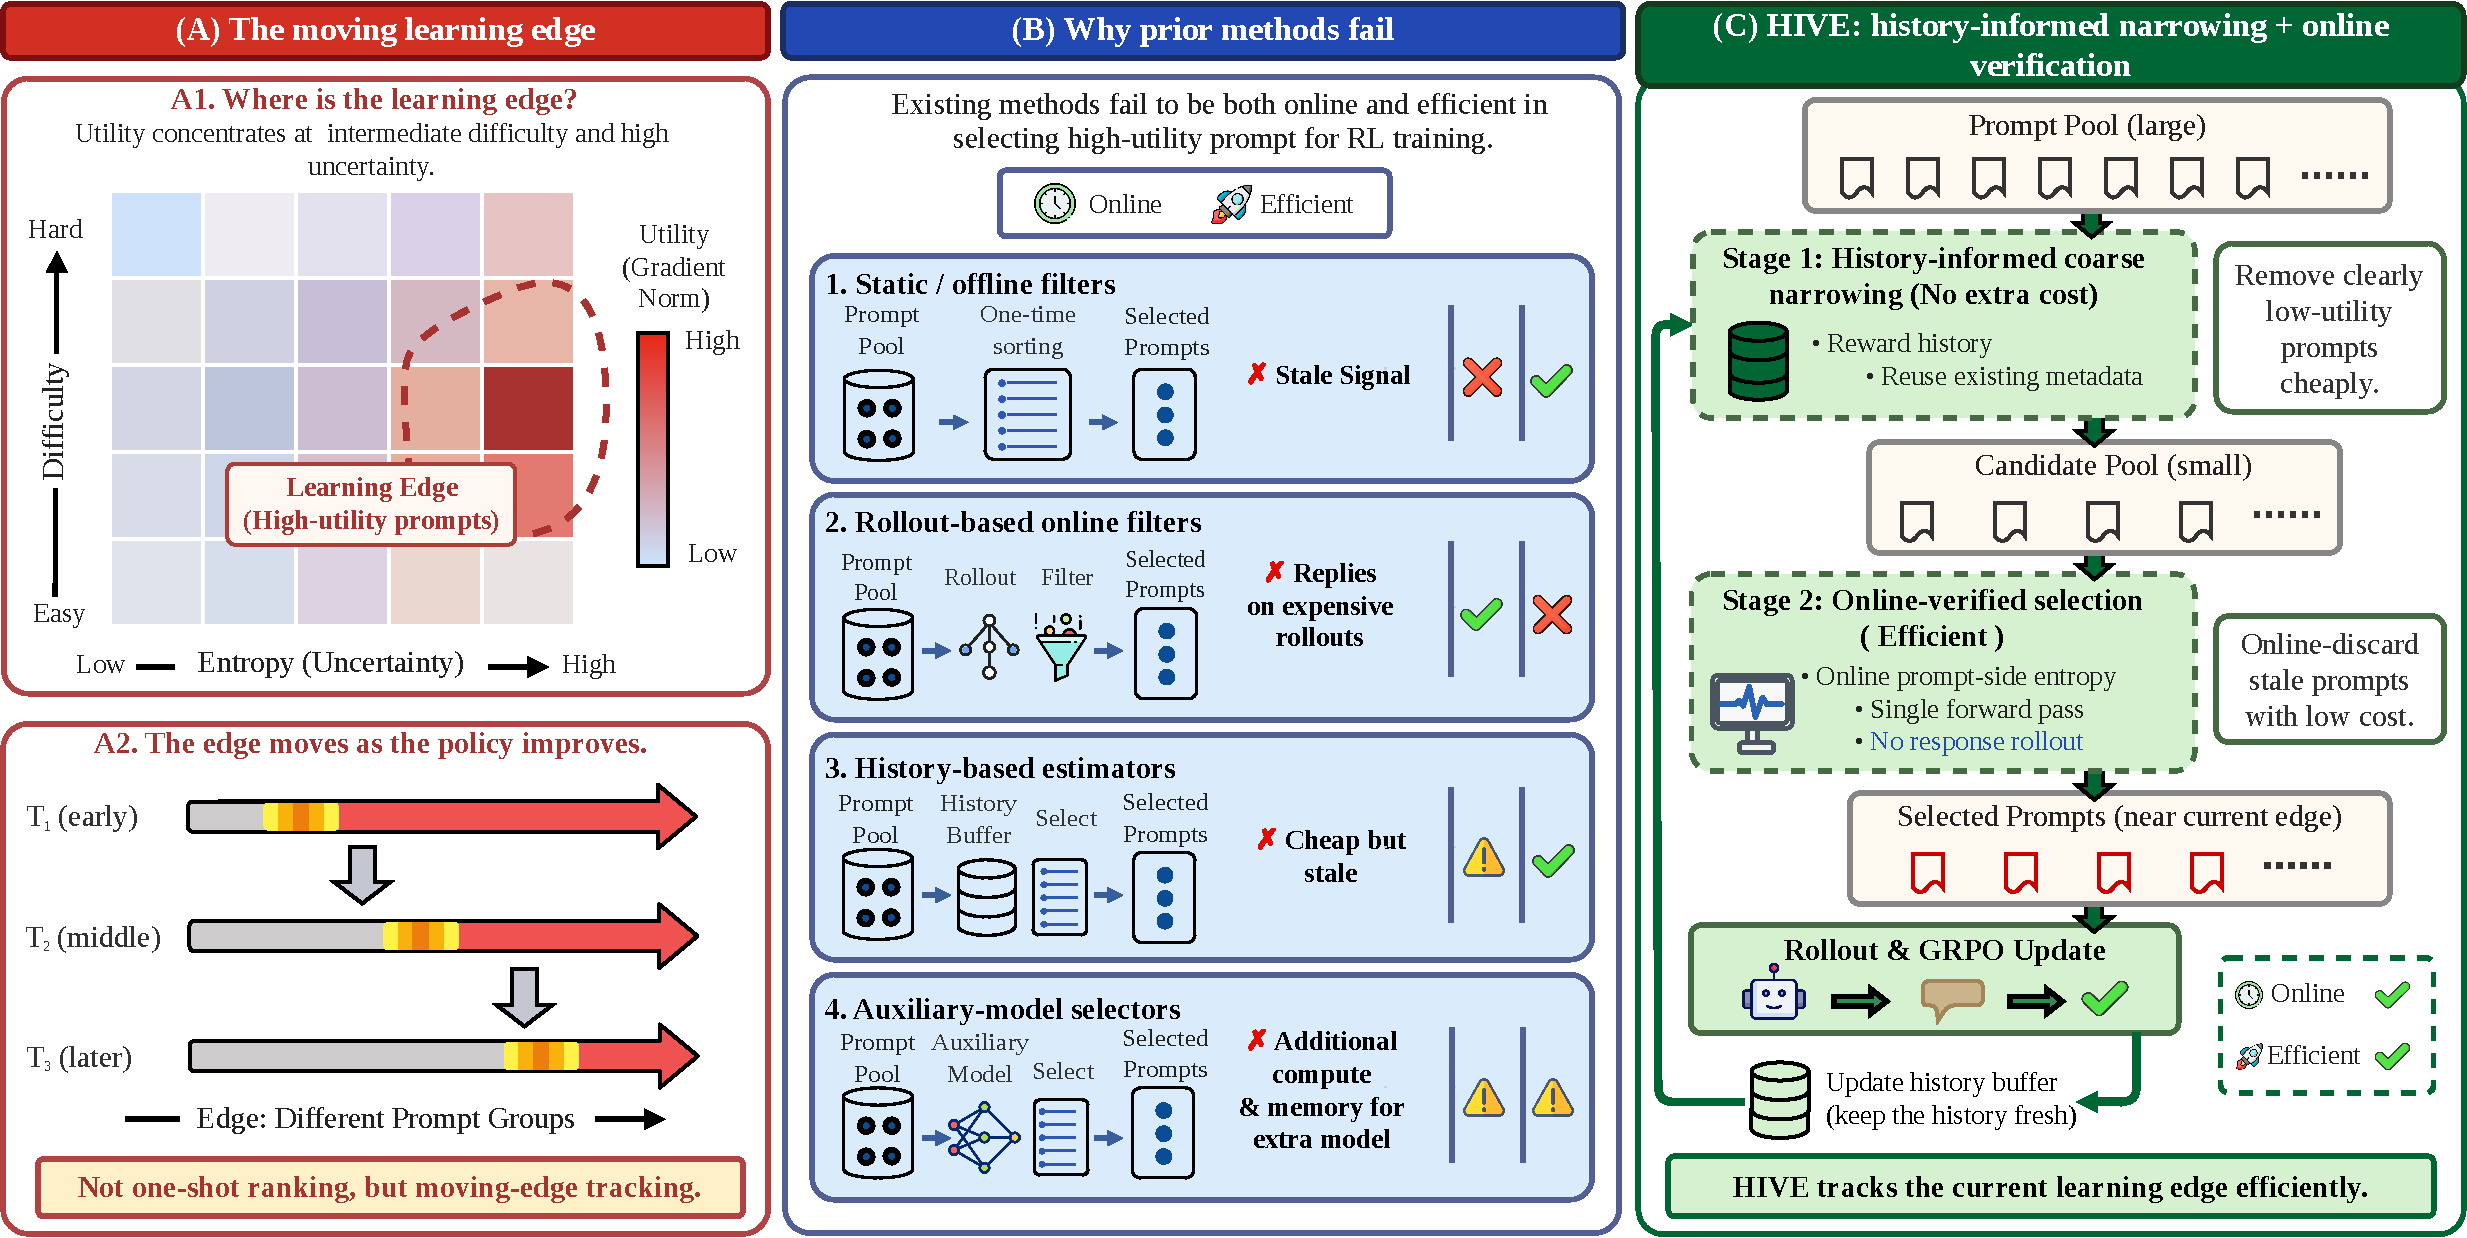
\includegraphics[width=0.98\linewidth]{figures/introduction/intro-fig-compare-motivate-1.pdf}
    \caption{\textbf{RLVR prompt selection is a moving-edge tracking problem.} (A) Utility concentrates at 
    intermediate difficulty and high uncertainty, and the learning edge is dynamic. 
    (B) Prior methods face limitations in efficiently selecting online high-utility prompts. (C) HIVE combines history-informed coarse narrowing with low-cost online 
    verification to track the current learning edge.}
    \label{fig:intro-compare-motivate}
    \vskip -0.2in
\end{figure}
% \red{1. re-write this caption 2.
%     delete precise. 3. redraw figure 3(d) to correspond to the A2 in figure 1. 4. shoud not be like curriculum, 
%     instead the utility of prompts across different step should be varying.}

\section{Introduction}
\label{sec:introduction}
Reinforcement Learning (RL) has emerged as a prevalent paradigm for fine-tuning large language models (LLMs), particularly for enhancing complex mathematical and logical reasoning capabilities~\cite{guo2025deepseek,yu2025dapo,tomihari2026learningdynamicsrlposttraining}. While advanced RL algorithms such as group relative policy optimization (GRPO)~\cite{shao2024deepseekmath} rely on rollout scaling to stabilize training and enhance model performance, they introduce a severe computational overhead~\cite{xu2025not,yu2025dapo,li2026stalefeedbackcoevolvingcritics}. In the training of those RL algorithms, a large portion of computational resources is wasted on generating rollouts for low-utility prompts that are either too trivial or too intractable for the current model. This results in vanishing gradients and wasted resources, providing no informative learning signal for model updates~\cite{zheng2025act,yu2025dapo,noukhovitch2025fasterICLR,verl2025}. Therefore, we investigate the following research question in this paper: \textit{how to identify prompts that are likely to produce useful gradients before rollout?}

Existing methods face limitations in efficiently selecting {high-utility} prompts in an online manner. Static or offline filters rank prompts before training using fixed heuristics, making them inexpensive but unable to adapt to the changing model during RL 
training~\cite{Wang2025ReinforcementLF,Li2025LIMRLI,ye2025limo}. Rollout-based online filters, such as dynamic sampling, better capture the current utility of each prompt by checking reward variance from newly generated responses~\cite{yu2025dapo,xu2025not,Chen2025LSPO,Ye2025PROF}. However, they already incur substantial rollout cost. History-based estimators such as GRESO~\cite{zheng2025act} avoid additional 
rollout cost by estimating prompt utility from past reward statistics, but those metadata becomes stale as the policy 
updates~\cite{zheng2025act,sun2025dots,li2026stalefeedbackcoevolvingcritics}. Auxiliary-model selectors, such as PCL~\cite{Gao2025PCL}, attach external or jointly trained predictors to estimate prompt difficulty or utility, introducing extra compute and memory during selection. 

% To understand what makes a prompt useful during RL training, we first conduct an empirical analysis of GRPO 
% training dynamics.  
% Among prompts with non-zero gradients, high response-side entropy prompts yield stronger learning progress at the same 
% rollout budget (Figure~\ref{fig:intro-a-b}b). More broadly, utility (\red{which we measured via length-normalized gradient norm}) concentrates at the intersection 
% of \red{intermediate difficulty} and high response-side entropy (Figure~\ref{fig:intro-a-b}c), which we term as 
% {learning edge}. However, the edge moves: prompts selected by those historical metadata quickly 
% lose real-time utility, whereas prompts verified under the current policy retain higher gradient norms 
% (Figure~\ref{fig:intro-a-b}a,\ref{fig:intro-a-b}d). Based on these observations, we conclude that an ideal prompt selection 
% framework for efficient LLM RL must be: \textbf{online} to track the moving learning edge, and \textbf{efficient} to avoid excessive overhead for selection.
% To identify what makes a prompt useful during RL training, we first empirically analyze GRPO training dynamics. Among prompts with non-zero gradients, those with high response-side entropy produce greater learning progress under the same rollout budget (Figure~\ref{fig:intro-a-b}b). More broadly, utility, measured by the length-normalized gradient norm, concentrates at the intersection of intermediate difficulty and high response-side entropy (Figure~\ref{fig:intro-a-b}c), which we refer to as the learning edge. However, this edge is dynamic: prompts selected using historical metadata quickly lose real-time utility, whereas prompts verified under the current policy retain higher gradient norms (Figure~\ref{fig:intro-a-b}a,\ref{fig:intro-a-b}d). These observations suggest that an effective prompt selection framework for efficient LLM RL should be \textbf{online}, to track the moving learning edge, and \textbf{efficient}, to avoid excessive selection overhead.
To identify what makes a prompt useful during RL training, we first empirically analyze GRPO training dynamics. Among prompts with non-zero gradients, those with high response-side entropy produce greater learning progress under the same rollout budget (Figure~\ref{fig:intro-high-entropy}). More broadly, utility, measured by the length-normalized gradient norm, concentrates at the intersection of intermediate difficulty and high response-side entropy (Figure~\ref{fig:intro-learning-edge}), which we refer to as the learning edge. However, this edge is dynamic: prompts selected using historical metadata quickly lose real-time utility, whereas prompts verified under the current policy retain higher gradient norms (Figures~\ref{fig:intro-history-staleness}); prompts move substantially among High, Low, and Zero utility classes across training steps (Figure~\ref{fig:intro-utility-shift}). These observations suggest that an effective prompt selection framework for efficient LLM RL should be \textbf{online}, to track the moving learning edge, and \textbf{efficient}, to avoid excessive selection overhead.
% To identify what makes a prompt useful during RL training, we first empirically analyze GRPO training dynamics. Among prompts with non-zero gradients, those with high response-side entropy produce greater learning progress under the same rollout budget (Figure~\ref{fig:intro-high-entropy}). More broadly, utility, measured by the length-normalized gradient norm, concentrates at the intersection of intermediate difficulty and high response-side entropy (Figure~\ref{fig:intro-learning-edge}), which we refer to as the learning edge. However, this edge is dynamic: prompts selected using historical metadata quickly lose real-time utility, whereas prompts verified under the current policy retain higher gradient norms (Figure~\ref{fig:intro-history-staleness}); prompts also move substantially among High, Low, and Zero utility classes across training steps (Figure~\ref{fig:intro-utility-shift}). These observations suggest that an effective prompt selection framework for efficient LLM RL should be \textbf{online}, to track the moving learning edge, and \textbf{efficient}, to avoid excessive selection overhead.


% To understand what makes a prompt useful for RL training, we first empirically examine GRPO training dynamics. Among prompts with non-zero gradients, those with higher response-side entropy yield greater learning progress under the same rollout budget (Figure~\ref{fig:intro-high-entropy}). More generally, utility, measured by the length-normalized gradient norm, is concentrated where intermediate difficulty and high response-side entropy intersect (Figure~\ref{fig:intro-learning-edge}); we refer to this region as the \emph{learning edge}. However, this edge shifts over time: prompts selected using historical metadata rapidly lose real-time utility, whereas prompts verified under the current policy maintain higher gradient norms (Figure~\ref{fig:intro-history-staleness}). Moreover, prompts frequently transition among High-, Low-, and Zero-utility classes throughout training (Figure~\ref{fig:intro-utility-shift}). These findings suggest that an effective prompt selection framework for efficient LLM RL should be both \textbf{online}, to track the moving learning edge, and \textbf{efficient}, to minimize selection overhead.

Based on previous analysis, we propose \textbf{HIVE} (\textbf{H}istory-\textbf{I}nformed \textbf{V}erification of the learning \textbf{E}dge), a dual-stage 
framework for rollout-efficient RLVR (Figure~\ref{fig:framework}). HIVE first performs history-informed coarse narrowing using 
reward trajectories and response-side entropies accumulated from previous training steps. This stage targets efficiency by retaining exploration probability for prompts that are around the edge. HIVE then utilizes prompt entropy as a high-fidelity and efficient proxy to perform online verification under the current policy, filtering stale candidates before the rollout phase.
% HIVE then performs online verification with prompt-side entropy 
% computed under the current policy. This stage restores online precision and filters 
% stale candidates before the rollout phase.

% Evaluation for HIVE is conducted across multiple reasoning benchmarks (e.g., {math, coding, and tool calling}) and models: Qwen3-4B~\cite{yang2025qwen3technicalreport}, 
Evaluation for HIVE is conducted across multiple reasoning benchmarks (e.g., math and tool calling) and models: Qwen3-4B-Base~\cite{yang2025qwen3technicalreport}, 
Qwen2.5-Math-1.5B/7B~\cite{yang2024qwen25mathtechnicalreportmathematical}, DeepSeek-R1-Distill-Qwen-1.5B~\cite{guo2025deepseek}, 
% Qwen2.5-14B/32B~\cite{qwen2.5-large}, and Llama-3.2-3B-Instruct~\cite{grattafiori2024llama3}. HIVE maintains comparable or better accuracy than Dynamic Sampling~\cite{yu2025dapo}, Pre-filter, GRESO~\cite{zheng2025act}, and PCL~\cite{Gao2025PCL} while using fewer rollouts, achieving up to \textbf{3.8$\times$ speedup in rollout} and \textbf{2.3$\times$ faster total training time} for models like Qwen2.5-Math-7B. Finally, we show that HIVE drastically lowers computational overhead, reducing rollouts by \textbf{up to 9.2 million} while consistently maintaining or even exceeding the reasoning accuracy of strong selection baselines across DAPO+MATH, Open-R1, and larger Qwen2.5 model scales.
Qwen2.5-14B/32B~\cite{qwen2.5-large}, and Llama-3.2-3B-Instruct~\cite{grattafiori2024llama3}. HIVE significantly outperforms 
baselines like Dynamic Sampling~\cite{yu2025dapo}, GRESO~\cite{zheng2025act} and PCL~\cite{Gao2025PCL}, achieving up to \textbf{2.3$\times$ faster total training time} for models like Qwen2.5-Math-7B. Finally, we show that HIVE lowers computational 
overhead, achieving \textbf{up to 9.2 million rollouts reduction} while consistently maintaining the reasoning performance. Beyond mathematical reasoning, HIVE also attains the best BFCL-V2 tool-calling score while using \textbf{4.8$\times$ fewer rollouts} than Dynamic Sampling, suggesting that moving-edge tracking extends to verifiable tool-use tasks.
%Besides, \red{the studies on coding and tool-calling tasks also show the generality of HIVE beyond math reasoning.}
% Our contributions are threefold:
% \begin{itemize}[topsep=2pt,itemsep=1pt,leftmargin=*]
%     and efficient required for practical selection. 
%     \item We propose HIVE, a dual-stage selector that combines zero-cost history-informed narrowing with low-cost online verification. 
%     \item We demonstrate across multiple tasks and model scales that HIVE significantly reduces rollout and wall-clock training costs while 
%     preserving or improving performance on those tasks.
% \end{itemize}
% Table 2 (Open-R1) and Figure 5 (Qwen2.5-14B/32B) merged into a single
% top-of-page side-by-side float for compactness.
% \documentclass{article}
% \usepackage{booktabs}
% \usepackage{graphicx}
% \usepackage{caption} % 必须引入，用于支持 \captionof

% \begin{document}

\begin{table*}[t]
    \centering
    % ==========================
    % 左侧：表格 (占约 64% 宽度)
    % ==========================
    % \hfill % 中间弹性间距
    % ==========================
    % 右侧：图片 (占约 32% 宽度)
    % ==========================
    \begin{minipage}[c]{0.255\textwidth}
        \centering
        % 插入图片
        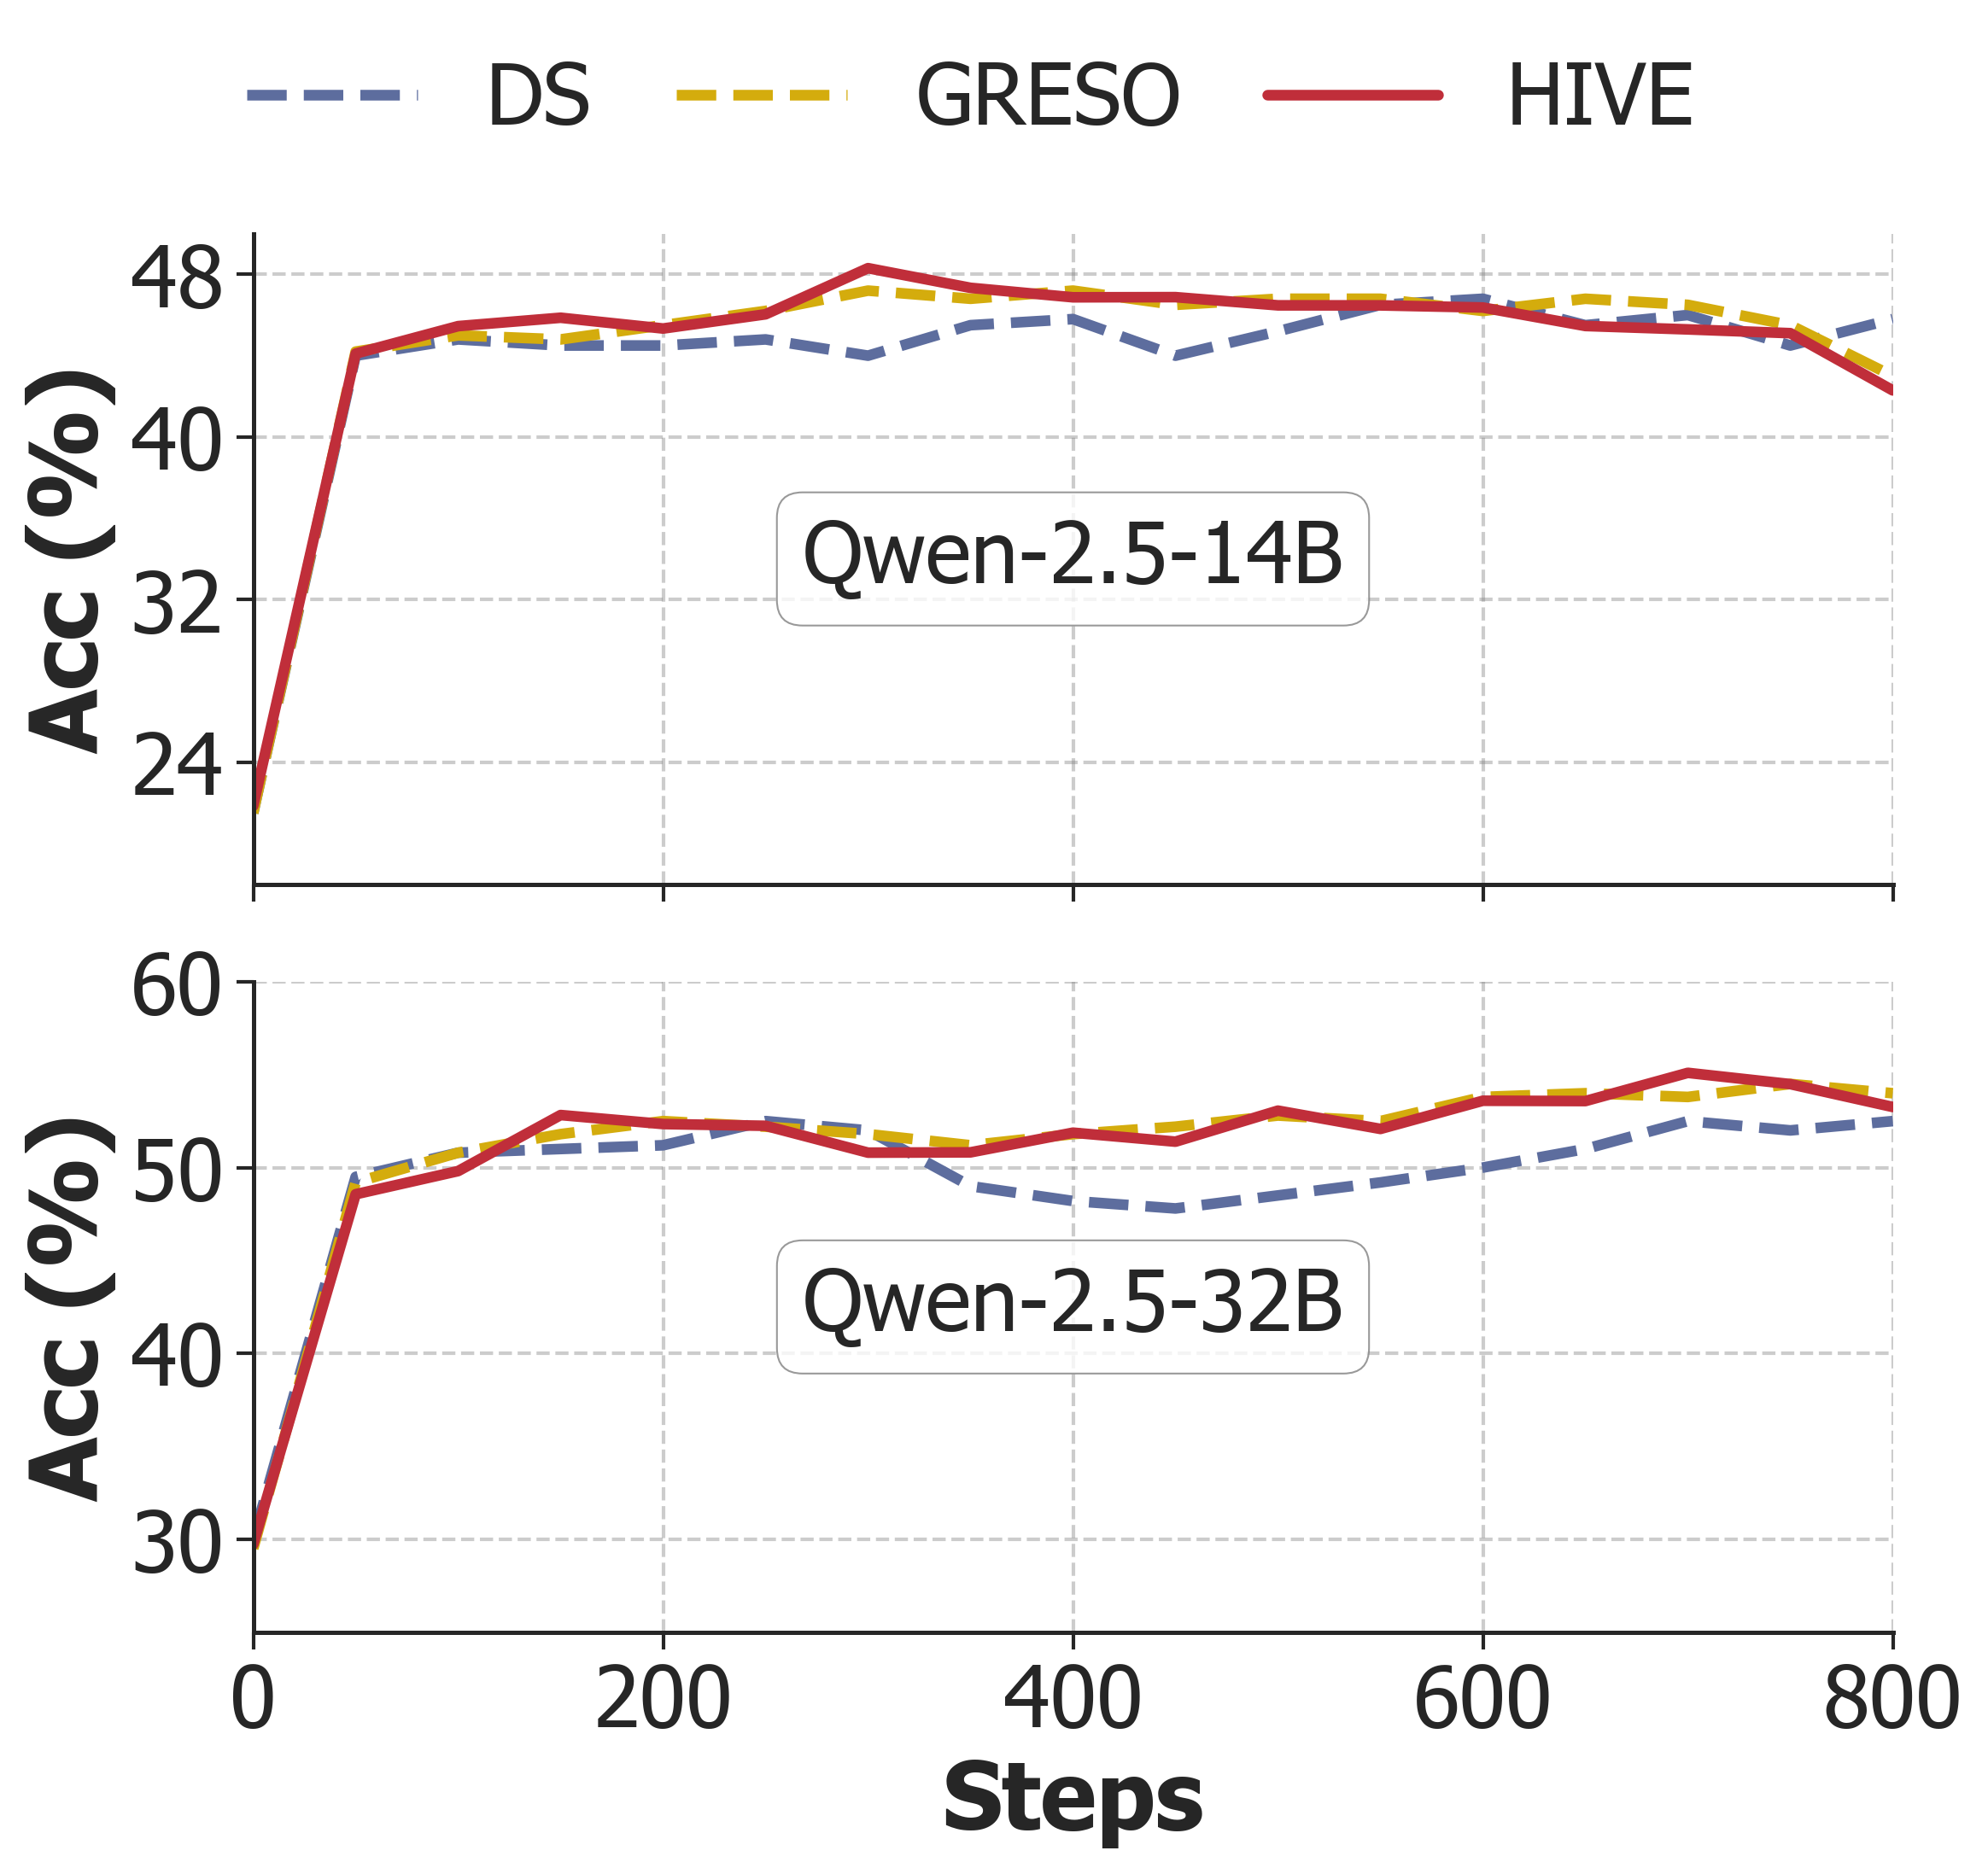
\includegraphics[width=\linewidth]{figures/experiment/12-scale-to-14b-32b_styled_vertical.png}
        % 使用 captionof{figure} 给图片正确编号
        \captionof{figure}{Scaling up to Qwen2.5-14B/32B.}
        \label{fig:scale_14b_32b}
    \end{minipage}
    \hfill
        \begin{minipage}[c]{0.735\textwidth}
        \centering
        \caption{Performance (\%) and rollout comparison of Qwen2.5-Math-1.5B and Qwen2.5-Math-7B trained on Open-R1.}
        \label{tab:openr1-main-exp}
        
        % 使用 resizebox 确保宽表格能完美放入左侧空间
        \resizebox{\linewidth}{!}{
            \begin{tabular}{c|cccccc|c|c}
            \toprule
            {Method} & {Math500} & {AIME24} & {AMC} & {Gaokao} & {Miner.} & {Olymp.} & {Avg.} & {\#Rollout} \\
            \midrule
            
            % Block 1: Qwen2.5-Math-1.5B
            \multicolumn{9}{c}{{\textit{Qwen2.5-Math-1.5B}}} \\
            \midrule
            DS    & 77.1 & 16.7 & 50.3 & 65.5 & 30.9 & 39.7 & 46.7 & 3.8M (1.0$\times$) \\
            GRESO & 76.1 & 20.0 & 50.6 & 65.1 & 30.0 & 39.2 & 46.8 & 1.6M (2.4$\times$)\\
            HIVE  & 76.9 & 18.3 & 48.7 & 65.4 & 30.1 & 40.3 & 46.6 & \best{{1.5M} (2.5$\times$)} \\
            \midrule
            
            % Block 2: Qwen2.5-Math-7B
            \multicolumn{9}{c}{{\textit{Qwen2.5-Math-7B}}} \\
            \midrule
            DS    & 82.8 & 34.2 & 63.5 & 67.3 & 35.7 & 46.3 & 55.0 & 11.4M (1.0$\times$) \\
            GRESO & 82.3 & 35.0 & 64.4 & 66.8 & 36.5 & 45.7 & 55.1 & 3.4M (3.4$\times$) \\
            HIVE  & 82.6 & 36.7 & 63.9 & 66.7 & 36.2 & 45.9 & 55.3 & \best{2.5M (4.7$\times$)} \\
            \bottomrule
            \end{tabular}
        }
    \end{minipage}
    \vskip -0.2in
\end{table*}
% \end{document}


\best{HIVE preserves accuracy while reducing rollouts.}
We compare HIVE against Dynamic Sampling (DS)~\cite{yu2025dapo}, a rollout-based online filter, and GRESO~\cite{zheng2025act}, a history-based selector. Table~\ref{tab:model_performance} reports results on DAPO+MATH across four model families. HIVE consistently uses fewer rollouts than both baselines while maintaining comparable average accuracy. On Qwen2.5-Math-7B, HIVE reduces rollouts by 70\% compared with DS (13.1M to 3.9M) and achieves the highest average accuracy (59.7\% vs. 57.8\% for DS and 58.6\% for GRESO), reaching comparable accuracy with substantially fewer generated responses.

\best{The gains transfer across datasets and model scales.}
Table~\ref{tab:openr1-main-exp} evaluates Qwen2.5-Math-1.5B/7B on Open-R1. HIVE again keeps comparable or better average accuracy while reducing rollouts, reaching 4.7$\times$ fewer rollouts than DS on Qwen2.5-Math-7B. Figure~\ref{fig:scale_14b_32b} extends the comparison to Qwen2.5-14B and Qwen2.5-32B. HIVE follows a similar convergence trajectory to DS and GRESO while requiring fewer rollouts; for Qwen2.5-14B over 800 steps, HIVE uses 1.56M rollouts compared with 1.74M for GRESO and 3.45M for DS.

\best{Wall-clock savings come from rollout reduction, not hidden overhead.}
Table~\ref{tab:efficiency_cost} decomposes end-to-end training time. HIVE reduces rollout time by up to 3.8$\times$ and total training time by up to 23$\times$ over DS. On Qwen2.5-Math-7B, total training time drops from 198.4 hours (DS) and 112.3 hours (GRESO) to 85.8 hours (HIVE), while rollout time drops from 153.7 and 66.3 to 40.2.

\begin{wraptable}[10]{r}{0.4\textwidth}
    \vspace{-1.2em}
    % \vskip -0.2in
    \centering
    \caption{Performance comparison (\%) on tool calling tasks.}
    \label{tab:tool_calling}
    \small
    \setlength{\tabcolsep}{3.2pt}
    \renewcommand{\arraystretch}{0.92}
    \begin{tabular}{lcc}
        \toprule
        Method & BFCL-V2 & \#Rollout \\
        \midrule
        DS & 79.08 & 5.3M \\
        Pre-filter & 77.04 & 1.4M \\
        GRESO & 78.96 & 1.4M \\
        PCL & 76.84 & 1.4M \\
        HIVE & \best{79.26} & \best{1.1M} \\
        \bottomrule
    \end{tabular}
    \vspace{-1.2em}
    % \vskip -0.2in
\end{wraptable}
\noindent\best{Performance on tool calling tasks.} Besides, we also verify the effectiveness of HIVE on tool calling tasks. We train Qwen2.5-1.5B on 80\% prompts samples from BFCL-V2~\cite{gorilla-openfunctions-v2} and evaluate the performance on the remaining 20\% subset~\cite{guo2025sample}. As shown in Table~\ref{tab:tool_calling}, HIVE achieves the highest BFCL-V2 score, slightly exceeding DS (79.26 vs. 79.08) while using only 1.1M rollouts instead of 5.3M. This corresponds to a 4.8$\times$ rollout reduction relative to DS. Under the same low-rollout regime, HIVE also outperforms the static Pre-filter baseline, the history-only GRESO selector, and the auxiliary PCL selector. These results suggest that moving-edge tracking is not only specific to mathematical reward signals, but also applicable on tool-calling tasks, where HIVE continues to concentrate rollout compute on informative prompt.

\subsection{Mechanism Analysis: Efficiency and Moving-Edge Adaptation}
\label{subsec:further-experiment}
\begin{figure*}[t]
    \centering
        % 第四张图：Zero-Variance Ratio
    \begin{subfigure}[b]{0.24\textwidth}
        \centering
        % \includegraphics[width=\textwidth]{figures/experiment/9-zero-variance-ratio-comparison-smoothed.png}
        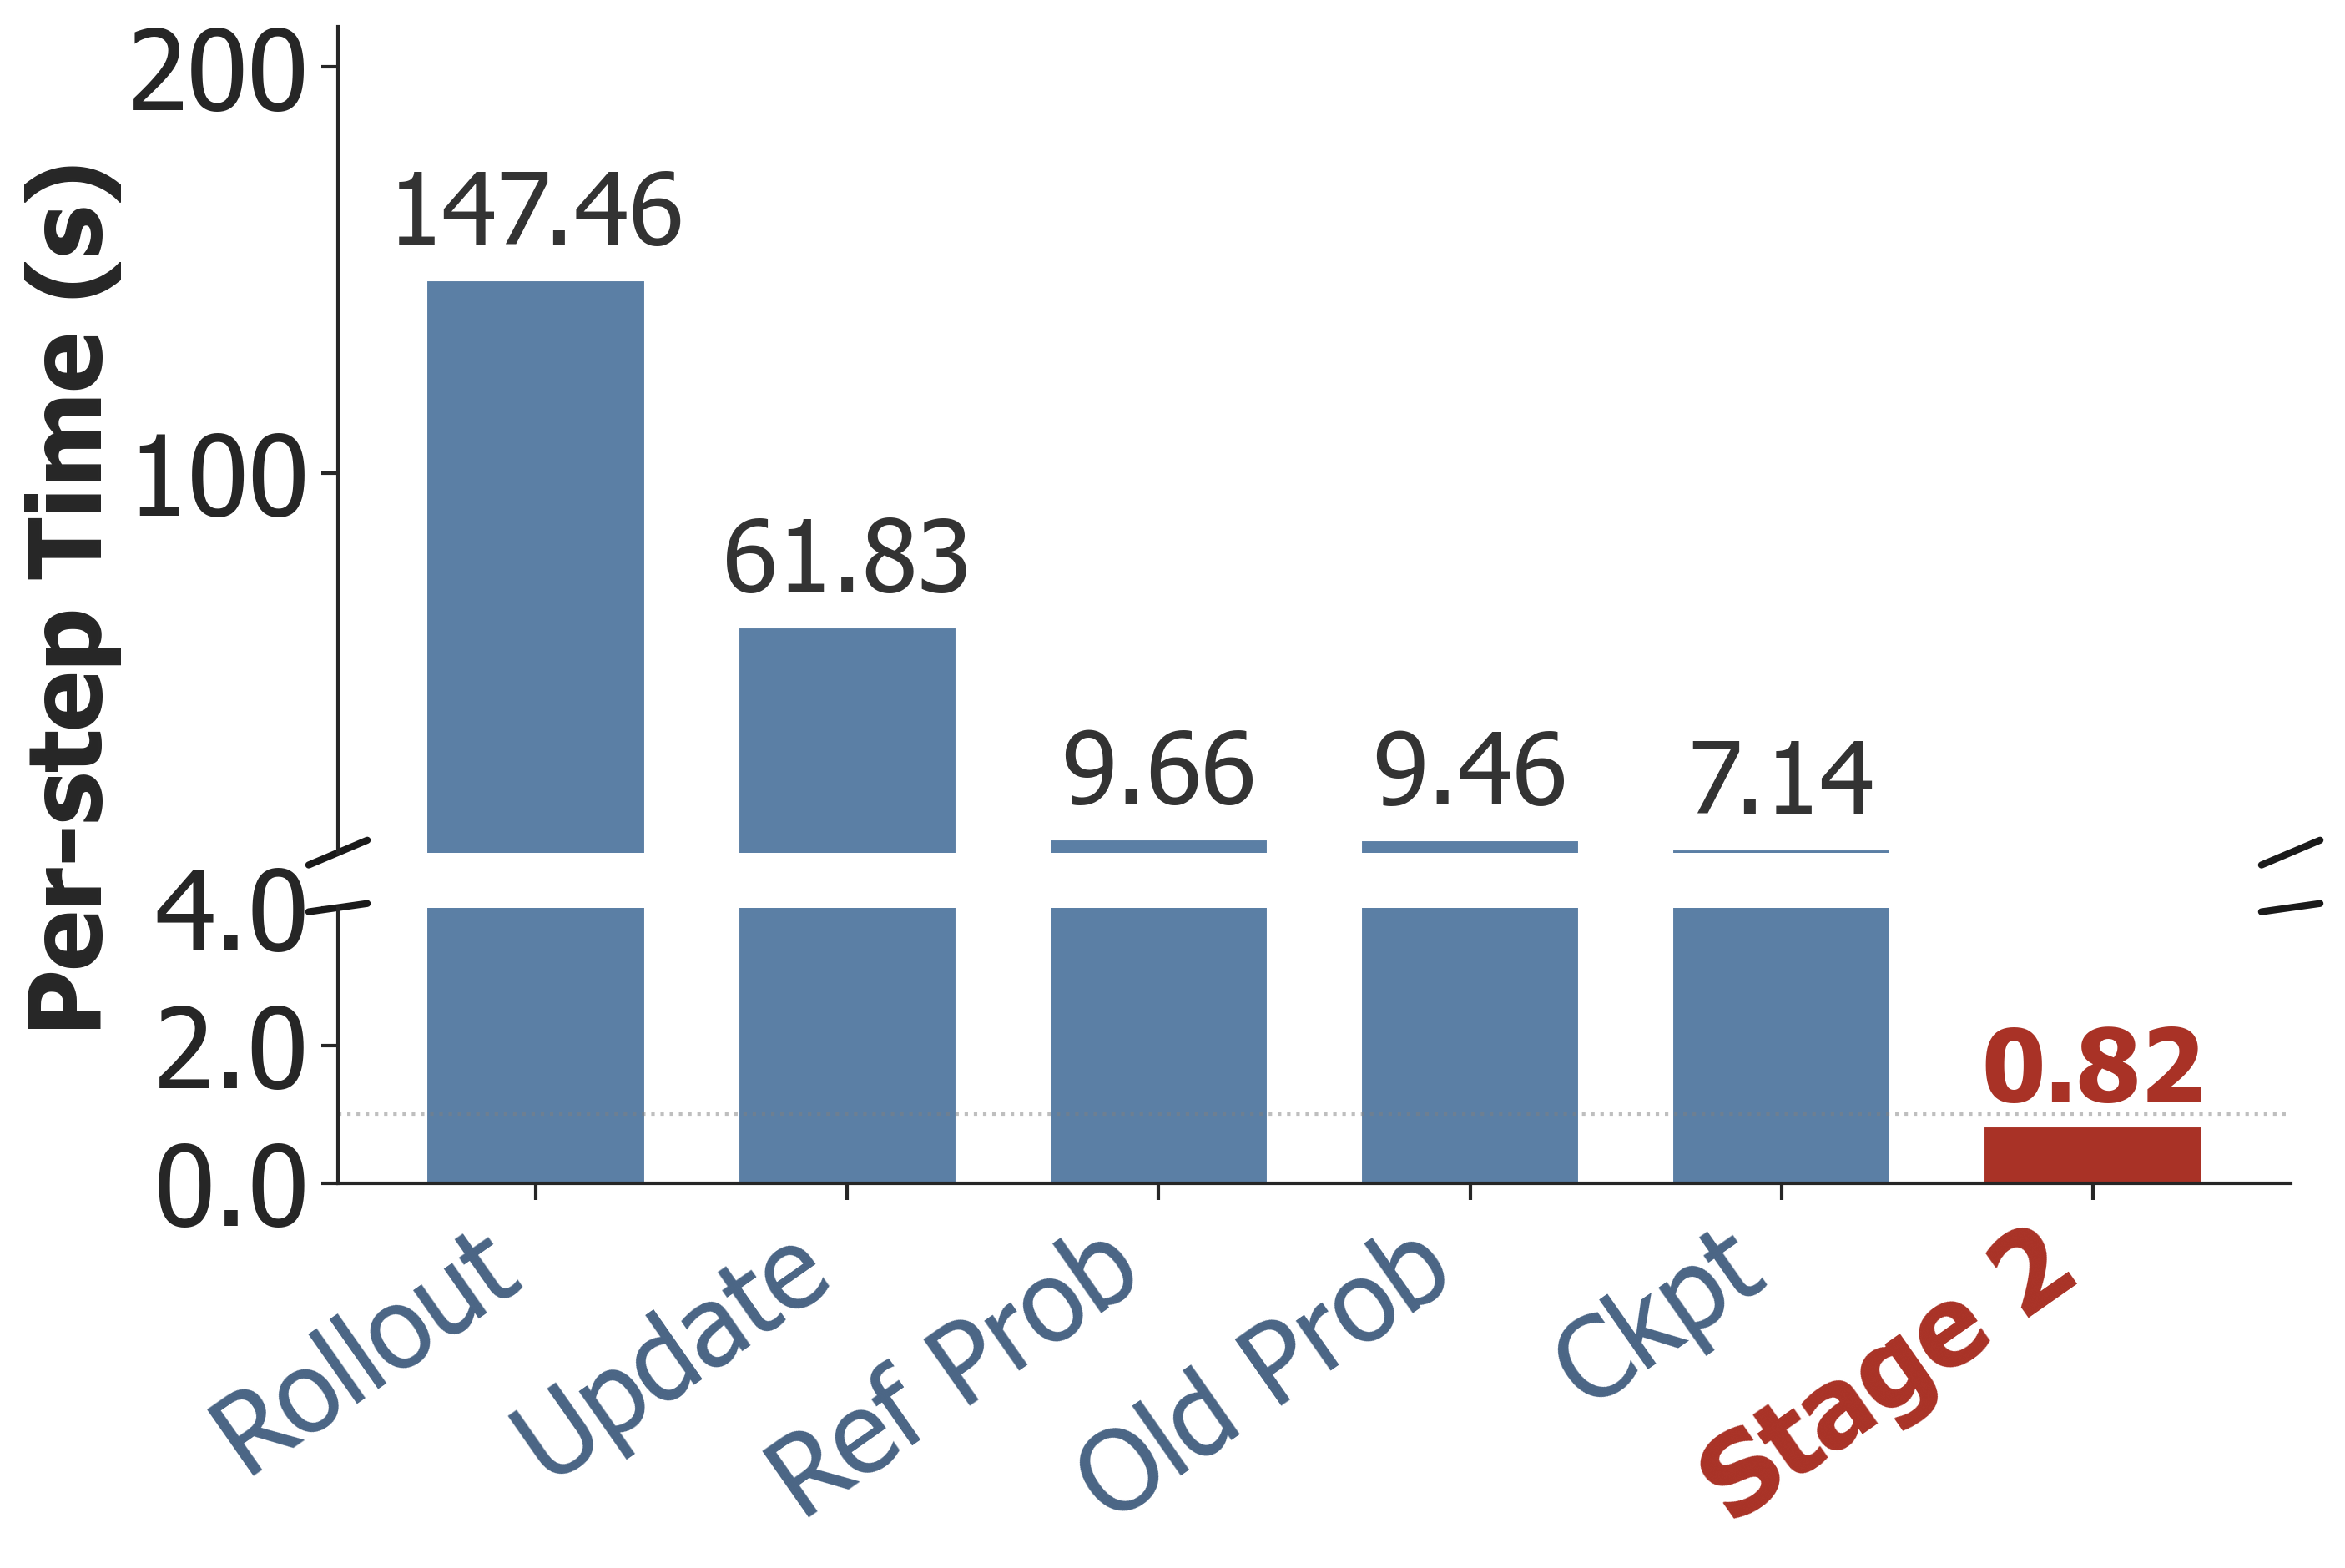
\includegraphics[width=\textwidth]{figures/experiment/5-broken_axis_styled.png}
        \caption{{Train-Time Breakdown}}
        \label{fig:per_step_time_analysis}
    \end{subfigure}
    % 第一张图：Rollout vs Time
    \begin{subfigure}[b]{0.24\textwidth}
        \centering
        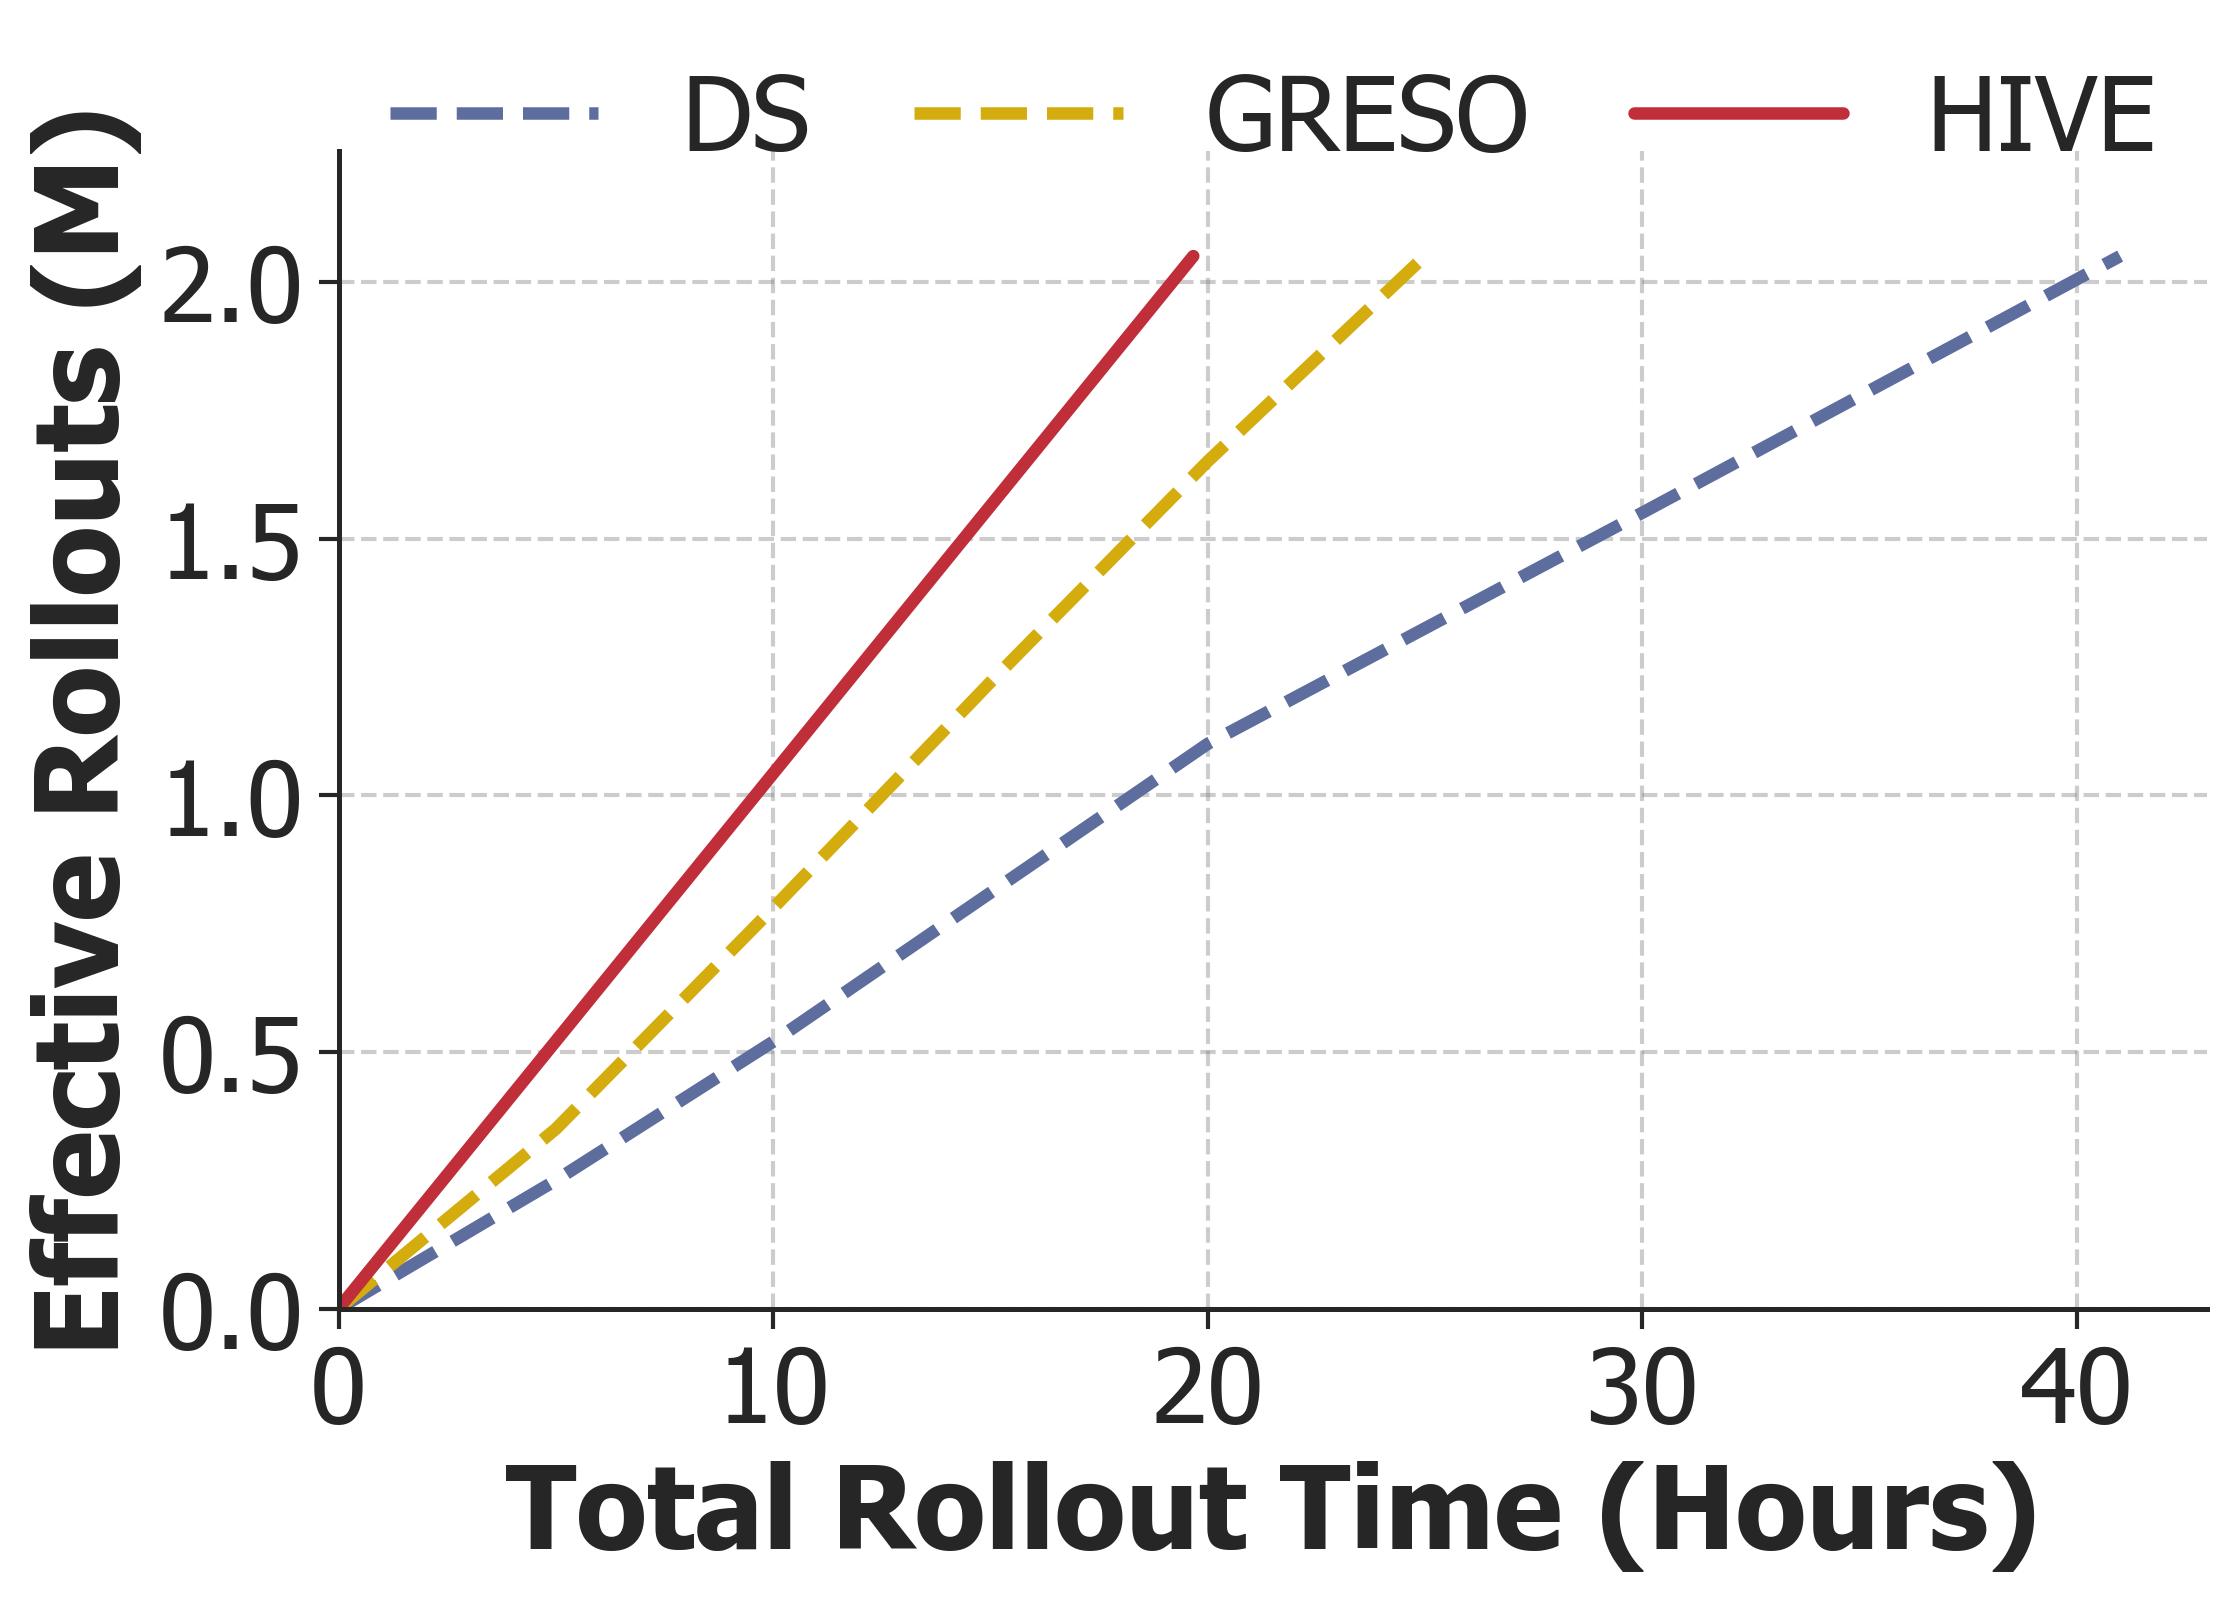
\includegraphics[width=\textwidth]{figures/experiment/11-total-rollout-time-VS-total-effective-rollouts.png}
        \caption{Efficiency Comparison}
        \label{fig:total_rollout}
    \end{subfigure}
    \hfill
    % 第二张图：Generation Time per Step
    \begin{subfigure}[b]{0.24\textwidth}
        \centering
        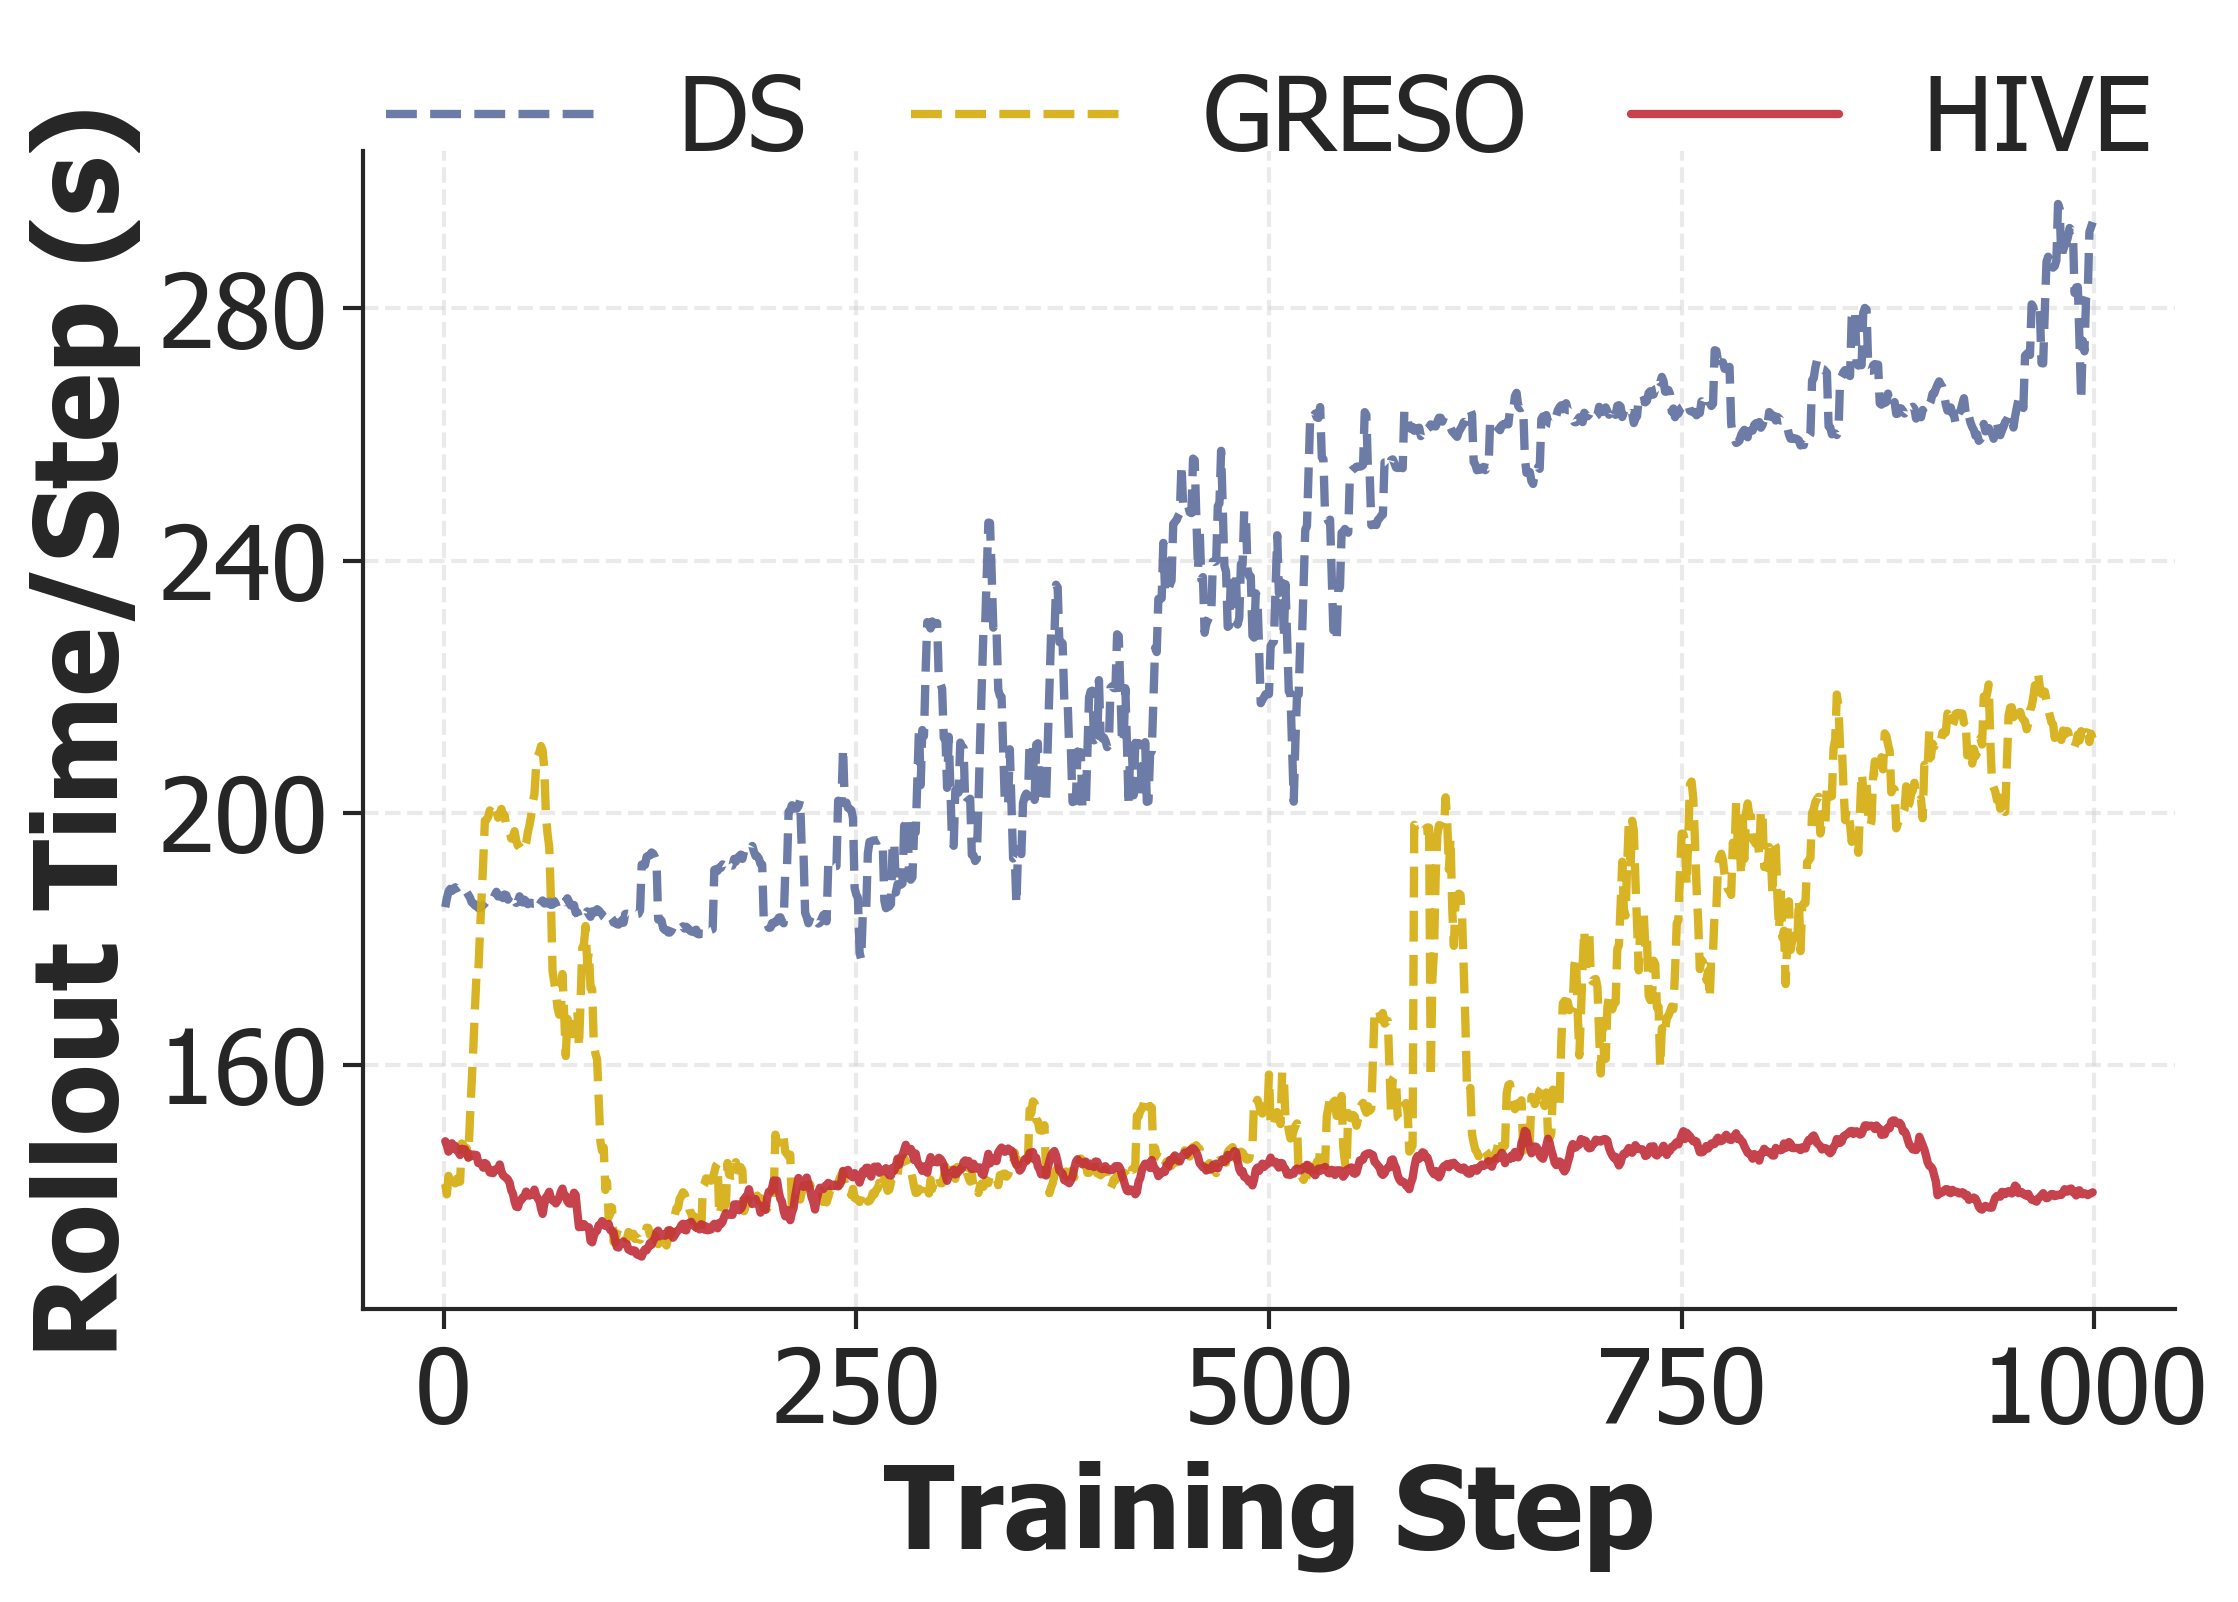
\includegraphics[width=\textwidth]{figures/experiment/10-rollout-time-per-step-comparison-smoothed.png}
        \caption{Generation Time}
        \label{fig:gen_time}
    \end{subfigure}
    \hfill
    % 第三张图：Rollouts per Step
    \begin{subfigure}[b]{0.24\textwidth}
        \centering
        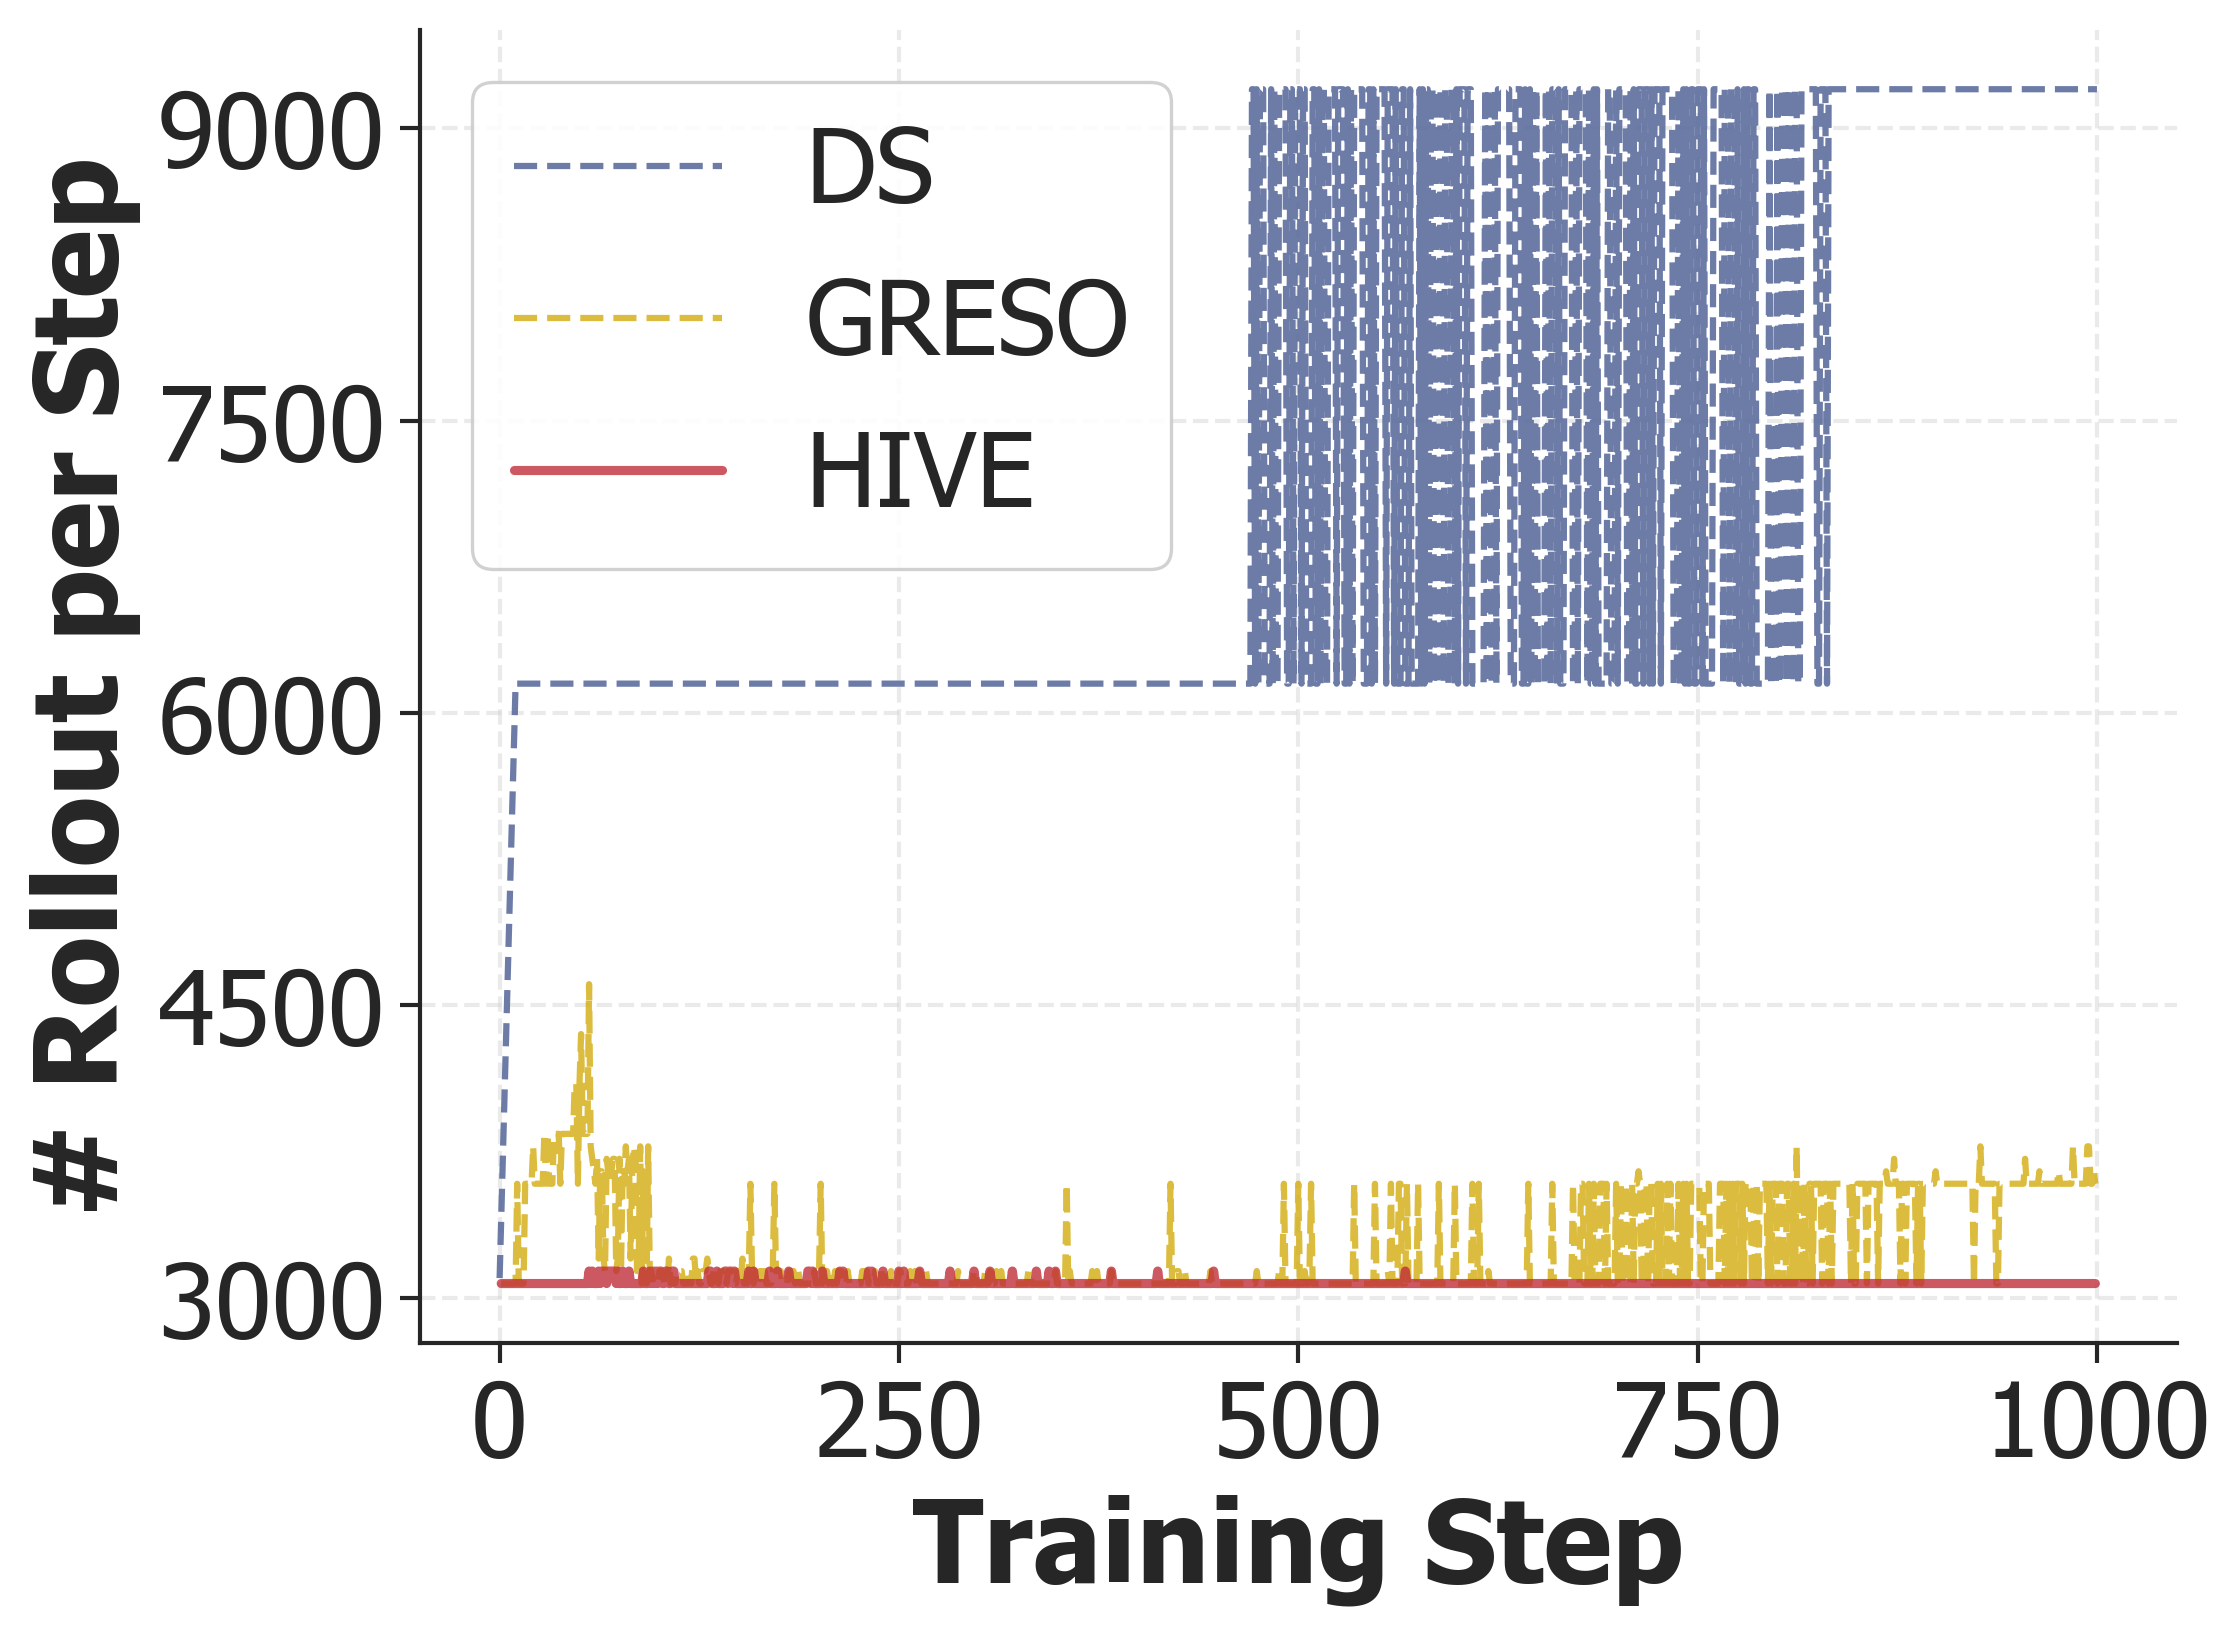
\includegraphics[width=\textwidth]{figures/experiment/8-per-step-rollout-comparison.png}
        \caption{Rollouts per Step}
        \label{fig:rollout_step}
    \end{subfigure}
    \hfill
    
    \caption{Efficiency analysis of Qwen2.5-Math-1.5B trained on DAPO+MATH. (a) Stage~2 prompt-side verification adds little time relative to rollout generation. (b) HIVE accumulates effective rollouts fastest per rollout hour. (c) HIVE maintains lower generation latency throughout training. (d) HIVE rolls out fewer prompt groups per step, concentrating compute on verified candidates.}
    \label{fig:further-analysis}
\end{figure*}


\best{Online verification is cheap enough to run before rollouts.}
Figure~\ref{fig:per_step_time_analysis} isolates the per-step overhead of Stage~2. Computing prompt-side entropy adds only 0.82 seconds, less than 0.4\% of the iteration time, while the rollout phase alone takes 147.46 seconds. This supports the efficiency side of the triad: HIVE gains online information without paying for response generation during selection.

\best{HIVE improves effective rollout throughput.}
Figure~\ref{fig:total_rollout} shows that HIVE accumulates effective rollouts per hour fastest. Figure~\ref{fig:gen_time} further shows that HIVE maintains low rollout-generation latency throughout training, while GRESO becomes slower later in training. This is consistent with metadata staleness: a history-only selector increasingly admits prompts that look useful in the log but no longer produce efficient current updates. Figure~\ref{fig:rollout_step} shows that HIVE also generates fewer rollout groups per step, concentrating compute on a smaller set of verified prompts near the current edge.

% Figure 5 is now combined with Table 2 in sections/exp-table-plux-figure.tex
% (\input-ed near the top of subsection "Main Results"); keeping the
% standalone variants here as comments for reference.
% \input{sections/figures/exp-scale-14b-32b}
% \input{sections/figures/exp-scale-14b-32b-vertical.tex}
% % Single-row top-of-page figure that fuses what used to be Figure 6
% % (zero-variance ratios on Easy / Hard) and Figure 7 (threshold entropy +
% % Stage 1/2 ablation) into one wide composite.
% %
% % The composite PDF is rendered by
% %   ICML2026-submission-figure-script-drawio-todo/wandb-figure/merge4_zerovar_component.py
% %
% % Sub-labels are produced via \phantomsubcaption from the `subcaption`
% % package, so existing \ref{fig:non-zero-diveregence-comparison},
% % \ref{fig:gamma_entropy} and \ref{fig:ablation} keep resolving — and we
% % additionally expose \ref{fig:zerovar_easy} / \ref{fig:zerovar_hard}.

% \begin{figure}[t]
%     \centering
%     \includegraphics[width=\linewidth]{figures/experiment/exp-merge4-zerovar-component.pdf}%
%     %
%     % Phantom sub-labels — invisible.  We anchor each one inside a zero-
%     % width subfigure so the subcaption counter is bumped for the label
%     % that follows it.  After all four panels are claimed, the figure-
%     % level \caption{} step the figure counter so the trailing
%     % \label{fig:non-zero-diveregence-comparison} binds to the figure
%     % number, not the last sub-letter.
%     %
%     \begin{subfigure}{0pt}\phantomsubcaption\label{fig:zerovar_easy}\end{subfigure}%
%     \begin{subfigure}{0pt}\phantomsubcaption\label{fig:zerovar_hard}\end{subfigure}%
%     \begin{subfigure}{0pt}\phantomsubcaption\label{fig:gamma_entropy}\end{subfigure}%
%     \begin{subfigure}{0pt}\phantomsubcaption\label{fig:ablation}\end{subfigure}%
%     %
%     \caption{\textbf{Zero-variance ratios and component analysis.}
%     (a)~Easy zero-variance ratio: HIVE keeps the lowest fraction of all-correct prompts throughout training.
%     (b)~Hard zero-variance ratio: HIVE rapidly drops below DS and tracks GRESO.
%     (c)~The Stage~2 median prompt-entropy threshold $\gamma$ adapts as the policy becomes more confident.
%     (d)~Removing either Stage~1 or Stage~2 worsens the accuracy--rollout tradeoff.\red{replace the figures to pdf}}%
%     \label{fig:non-zero-diveregence-comparison}
%     \vskip -0.08in
% \end{figure}

\begin{figure*}[t]
    \centering
    \begin{subfigure}[b]{0.24\textwidth}
        \centering
        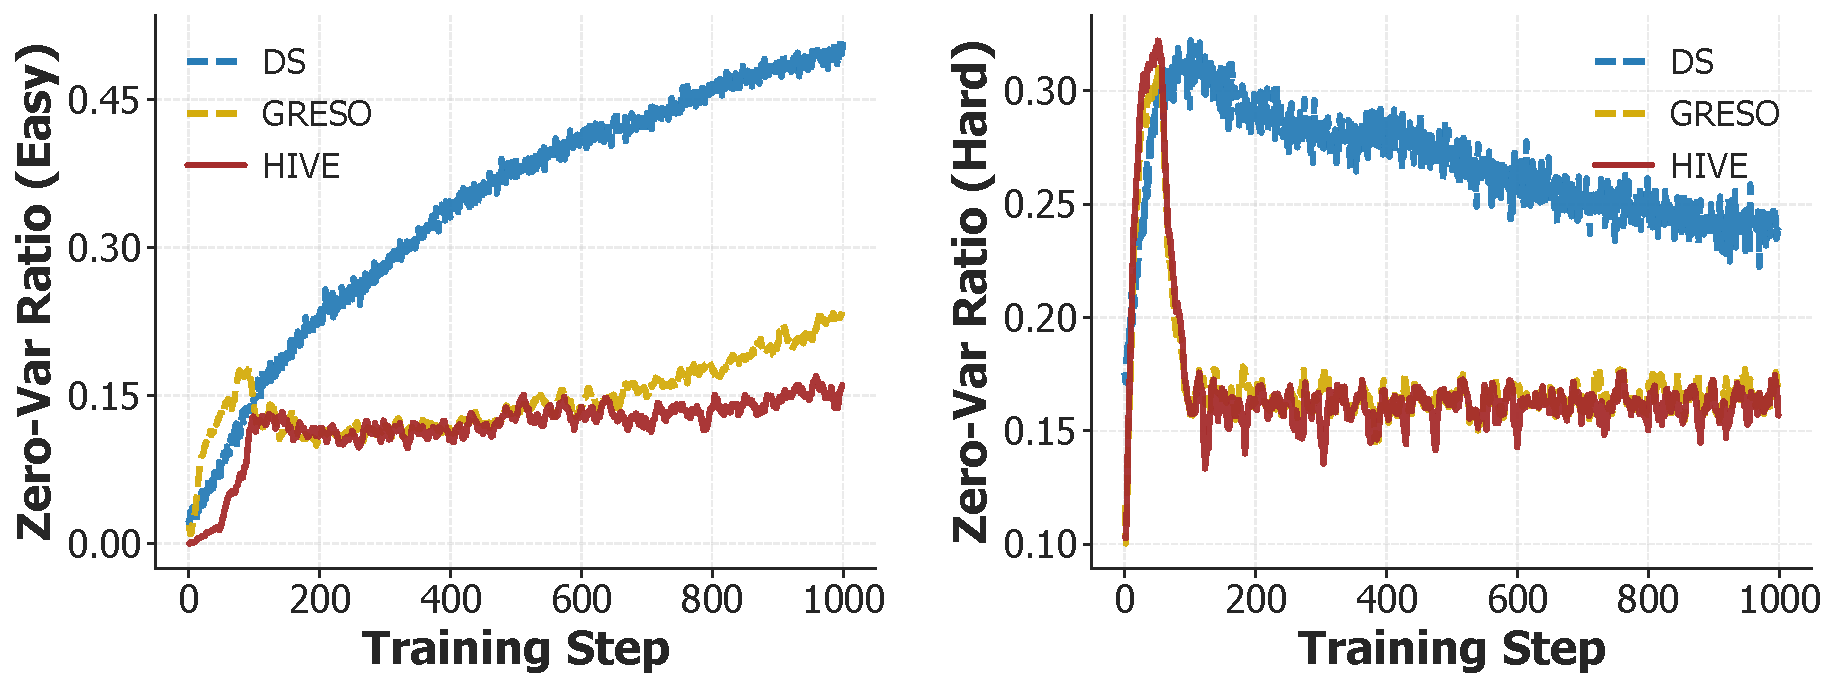
\includegraphics[width=\textwidth,trim=0 0 440.4bp 0,clip]{figures/experiment/fig6-zerovar-easy-hard-polished.pdf}
        \caption{Easy zero-variance}
        \label{fig:zerovar_easy}
    \end{subfigure}
    \hfill
    \begin{subfigure}[b]{0.24\textwidth}
        \centering
        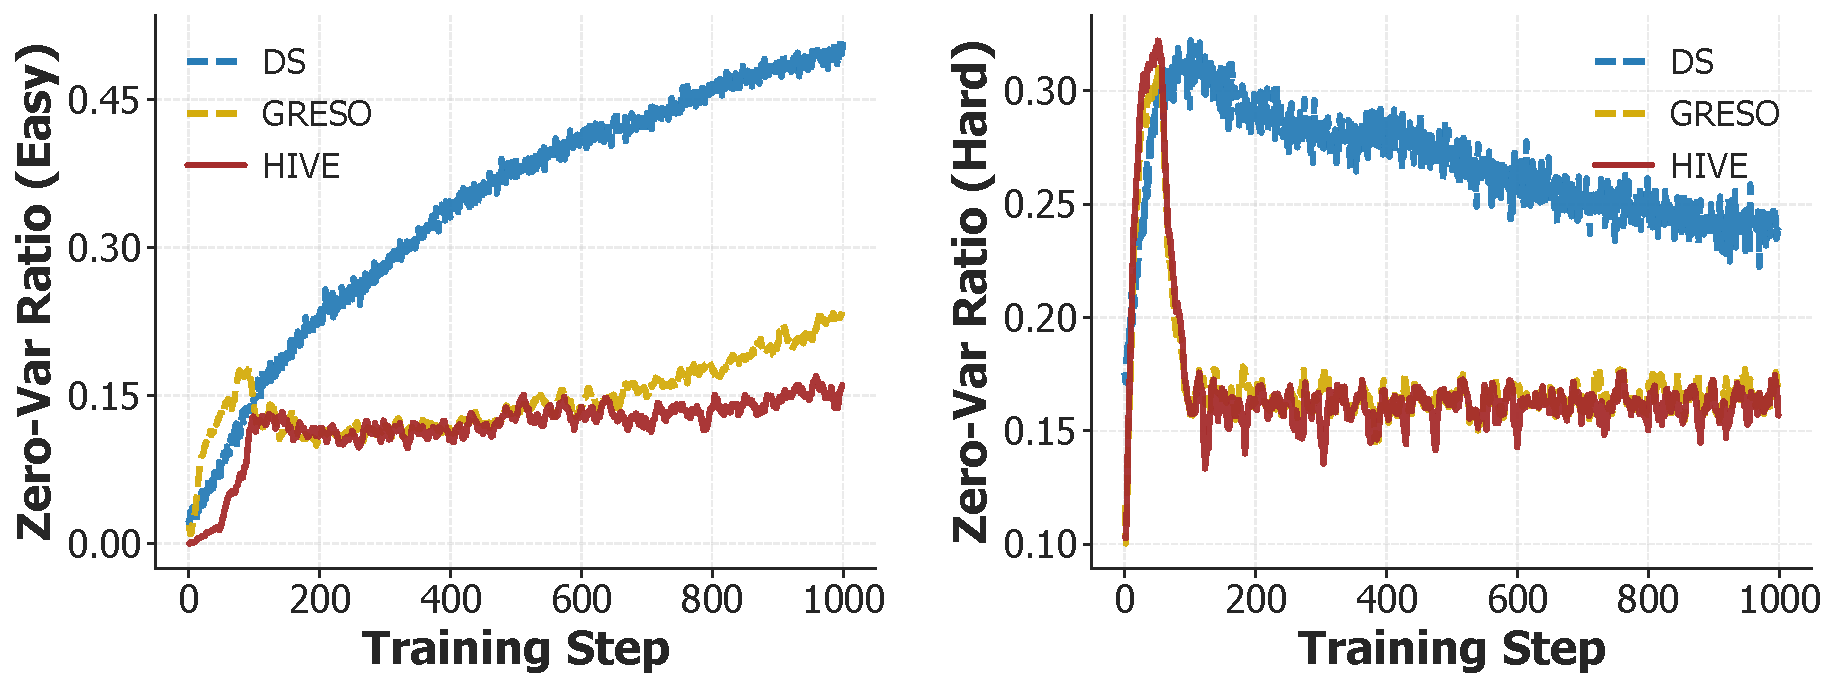
\includegraphics[width=\textwidth,trim=440.4bp 0 0 0,clip]{figures/experiment/fig6-zerovar-easy-hard-polished.pdf}
        \caption{Hard zero-variance}
        \label{fig:zerovar_hard}
    \end{subfigure}
    \hfill
    \begin{subfigure}[b]{0.24\textwidth}
        \centering
        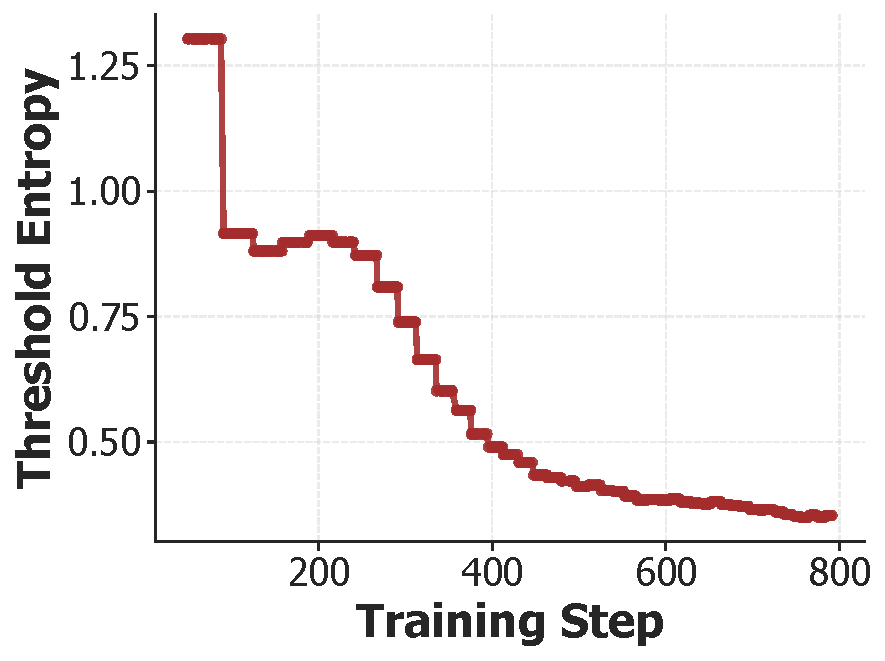
\includegraphics[width=\textwidth]{figures/experiment/fig6-gamma-entropy-polished.pdf}
        \caption{Entropy threshold}
        \label{fig:gamma_entropy}
    \end{subfigure}
    \hfill
    \begin{subfigure}[b]{0.24\textwidth}
        \centering
        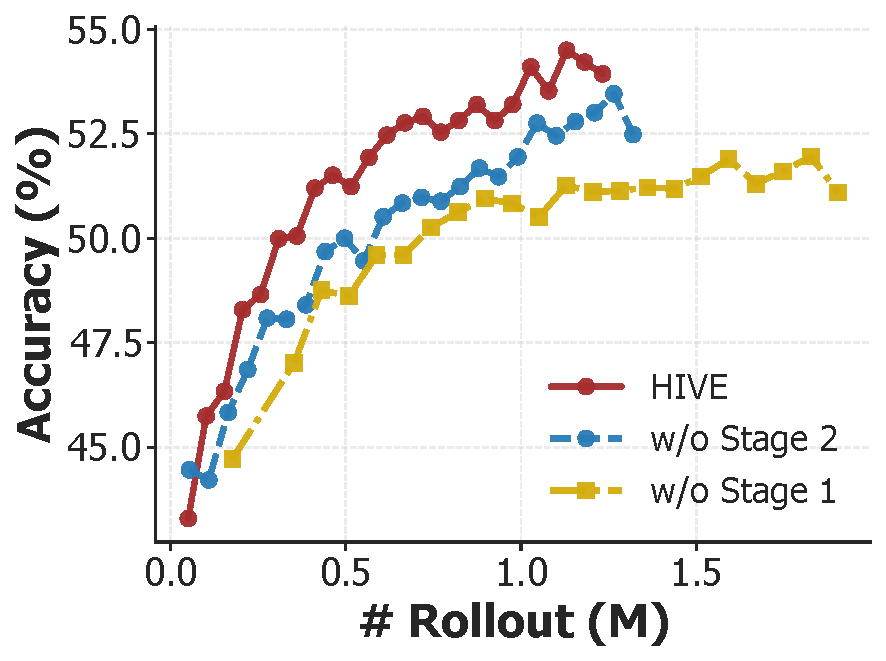
\includegraphics[width=\textwidth]{figures/experiment/fig6-stage-ablation-polished.pdf}
        \caption{Stage ablation}
        \label{fig:ablation}
    \end{subfigure}

    \caption{\textbf{Zero-variance ratios and component analysis.}
    (a)~Easy zero-variance ratio: HIVE keeps the lowest fraction of all-correct prompts throughout training.
    (b)~Hard zero-variance ratio: HIVE rapidly drops below DS and tracks GRESO.
    (c)~The Stage~2 median prompt-entropy threshold $\gamma$ adapts as the policy becomes more confident.
    (d)~Removing either Stage~1 or Stage~2 worsens the accuracy--rollout tradeoff.}%
    \label{fig:non-zero-diveregence-comparison}
    \vskip -0.08in
\end{figure*}

\best{HIVE rejects stale zero-variance prompts as training evolves.}
The zero-variance ratio measures how often selected prompts produce no informative gradient. Figures~\ref{fig:zerovar_easy} and~\ref{fig:zerovar_hard} show that DS wastes a large fraction of rollouts on easy zero-variance prompts as the model improves, while GRESO remains vulnerable to stale historical records. HIVE maintains a lower zero-variance ratio for both easy and hard prompts, indicating that online verification helps track the moving edge rather than relying on outdated metadata.

\subsection{Component Study: Why Both Stages Matter}
\label{subsec:exp-component-study}

\best{The entropy gate adapts with the current policy.}
Figure~\ref{fig:gamma_entropy} tracks the Stage~2 median threshold $\gamma$, which decreases as the model becomes more confident. This behavior is expected: as the policy improves, the prompt-side uncertainty distribution shifts, and a fixed threshold would either over-prune or admit stale prompts. The median gate keeps the verification rule relative to the current candidate pool. 
\best{The two-stage decomposition is necessary.}
Figure~\ref{fig:ablation} compares the full HIVE pipeline with variants that remove either stage. Without Stage~2, HIVE loses online precision and becomes more vulnerable to stale metadata. Without Stage~1, the verifier receives too many low-value candidates, reducing efficiency. The full method gives the best accuracy--rollout tradeoff, supporting the decomposition into efficient historical narrowing followed by online verification.
